%% LyX 2.0.7.1 created this file.  For more info, see http://www.lyx.org/.
%% Do not edit unless you really know what you are doing.
\documentclass[10pt,twoside,english]{mwart}
\usepackage[LGR,T1]{fontenc}
\usepackage[latin9]{inputenc}
\usepackage{listings}
\usepackage[a4paper]{geometry}
\geometry{verbose,tmargin=3cm,bmargin=2cm,lmargin=2cm,rmargin=2cm,headheight=1cm,headsep=1cm}
\pagestyle{headings}
\setcounter{tocdepth}{2}
\usepackage{color}
\usepackage{babel}
\usepackage{array}
\usepackage{float}
\usepackage{fancybox}
\usepackage{calc}
\usepackage{units}
\usepackage{textcomp}
\usepackage{multirow}
\usepackage{amsthm}
\usepackage{amsmath}
\usepackage{graphicx}
\usepackage[unicode=true,
 bookmarks=true,bookmarksnumbered=false,bookmarksopen=false,
 breaklinks=true,pdfborder={0 0 0},backref=false,colorlinks=false]
 {hyperref}
\hypersetup{pdftitle={Android Sensors Overview},
 pdfauthor={Carlo Antenucci}}

\makeatletter

%%%%%%%%%%%%%%%%%%%%%%%%%%%%%% LyX specific LaTeX commands.
\DeclareRobustCommand{\greektext}{%
  \fontencoding{LGR}\selectfont\def\encodingdefault{LGR}}
\DeclareRobustCommand{\textgreek}[1]{\leavevmode{\greektext #1}}
\DeclareFontEncoding{LGR}{}{}
\DeclareTextSymbol{\~}{LGR}{126}
%% Special footnote code from the package 'stblftnt.sty'
%% Author: Robin Fairbairns -- Last revised Dec 13 1996
\let\SF@@footnote\footnote
\def\footnote{\ifx\protect\@typeset@protect
    \expandafter\SF@@footnote
  \else
    \expandafter\SF@gobble@opt
  \fi
}
\expandafter\def\csname SF@gobble@opt \endcsname{\@ifnextchar[%]
  \SF@gobble@twobracket
  \@gobble
}
\edef\SF@gobble@opt{\noexpand\protect
  \expandafter\noexpand\csname SF@gobble@opt \endcsname}
\def\SF@gobble@twobracket[#1]#2{}
%% Because html converters don't know tabularnewline
\providecommand{\tabularnewline}{\\}

%%%%%%%%%%%%%%%%%%%%%%%%%%%%%% Textclass specific LaTeX commands.
\numberwithin{equation}{section}
\numberwithin{figure}{section}
\newenvironment{lyxcode}
{\par\begin{list}{}{
\setlength{\rightmargin}{\leftmargin}
\setlength{\listparindent}{0pt}% needed for AMS classes
\raggedright
\setlength{\itemsep}{0pt}
\setlength{\parsep}{0pt}
\normalfont\ttfamily}%
 \item[]}
{\end{list}}
\theoremstyle{plain}
\newtheorem{thm}{\protect\theoremname}
  \theoremstyle{definition}
  \newtheorem{example}[thm]{\protect\examplename}

%%%%%%%%%%%%%%%%%%%%%%%%%%%%%% User specified LaTeX commands.
\usepackage{colortbl}
\definecolor{maroon}{rgb}{0.5,0,0}
\definecolor{darkgreen}{rgb}{0,0.5,0}
\definecolor{gray}{RGB}{192, 192, 192}
\lstdefinelanguage{XML}
{
  basicstyle=\ttfamily\footnotesize,
  morestring=[b]",
  moredelim=[s][\bfseries\color{darkgreen}]{<}{\ },
  moredelim=[s][\bfseries\color{darkgreen}]{</}{>},
  moredelim=[l][\bfseries\color{darkgreen}]{/>},
  moredelim=[l][\bfseries\color{darkgreen}]{>},
  morecomment=[s]{<?}{?>},
  morecomment=[s]{<!--}{-->},
  commentstyle=\color{maroon},
  stringstyle=\color{blue},
  identifierstyle=\color{magenta}
}

\@ifundefined{showcaptionsetup}{}{%
 \PassOptionsToPackage{caption=false}{subfig}}
\usepackage{subfig}
\makeatother

  \providecommand{\examplename}{Example}
\providecommand{\theoremname}{Theorem}

\begin{document}

\author{ALMA MATER STUDIORUM - UNIVERSITY OF BOLOGNA}


\title{\vspace*{\fill}{\Huge{}Android Sensors Overview}\\
{\Huge{}~}\\
{\large{}Carlo Antenucci}\vspace*{\fill}}

\maketitle
\cleardoublepage{}

\tableofcontents{}

\newpage{}
\begin{abstract}
Most Android-powered device have several built-in sensors that measure
motion, orientation and other various enviromental condition, provide
raw data with high precision and accuracy, and are useful to monitor
three-dimensional device movement and positioning or monitor changes
in the near ambiental environment near a device.\\


Android platform supports three category of sensors:

\textbf{Motion~sensors}: measure acceleration and rotational forces
along three axis. This category includes \textit{accelerometer}, g\textit{ravity
sensor}, \textit{gyroscope} and \textit{rotational vector sensor}.

\textbf{Enviromental}~\textbf{sensors}: sensors included in this
category (\textit{barometer}, \textit{photometer} and \textit{thermometer})
measure various enviromental parameters such as temperature, pressure,
illumination, humidity.

P\textbf{osition~sensor}s: measure physical position of a device
using \textit{orientation sensor }and \textit{magnetometer}.\\


The access to a sensor and the raw sensor data acquisition are simplified
by using Android Sensor Framework\textbf{ }that provides several classes
and interfaces that helps developer to perform a large number of sensor-related
task.

This paper is based to the Adroid Developers sensors documentation\cite{androidDev}
and introduces the Android sensor framework and explains how to use
sensors using some examples.

All source code are available at \href{https://github.com/CarloAntenucci/Android-Sensors-Overview.git}{https://github.com/CarloAntenucci/Android-Sensors-Overview.git}
\newpage{}
\end{abstract}

\section{About Android Sensor Framework}


\subsection{Introduction to sensors}

The Android Sensor Framework lets access to access many type of sensors,
some of these are hardware-based (real sensors) and some are are software-based
(virtual sensors).

Hardware-based sensors are built into the device and they derive data
by directly measuring specific environmental properties, while software-based
sensors are not physical devices despite they mimic an hardware-based
sensor. This second group derive their data from one ore more of the
hardware-based sensors.

\begin{center}
\begin{table}[H]
\caption{Sensor types supported by the Android platform}


\centering{}%
\begin{tabular}{|>{\raggedright}m{0.3\columnwidth}|>{\raggedright}m{0.1\textwidth}|>{\raggedright}m{0.3\textwidth}|>{\raggedright}m{0.2\textwidth}|}
\hline 
\rowcolor{cyan}
\centering\textbf{Sensor} & \centering\textbf{Type} & \centering\textbf{Description} & \centering\textbf{Sensor fusion}\tabularnewline
\hline 
\hline 
\texttt{\footnotesize{}TYPE\_ACCELEROMETER} & {\footnotesize{}Hardware} & {\footnotesize{}Measures the acceleration force in $\nicefrac{m}{s^{2}}$
that is applied to a device on all three physical axes (x, y, and
z), including the force of gravity.} & \tabularnewline
\hline 
\texttt{\footnotesize{}TYPE\_GRAVITY} & {\footnotesize{}Software or Hardware} & {\footnotesize{}Measures the force of gravity in $\nicefrac{m}{s^{2}}$
that is applied to a device on all three physical axes (x, y, and
z).} & {\footnotesize{}If it is software uses Accelerometer to derive data}\tabularnewline
\hline 
\texttt{\footnotesize{}TYPE\_GYROSCOPE} & {\footnotesize{}Hardware} & {\footnotesize{}Measures a device's rate of rotation in $\nicefrac{rad}{s}$
that is applied to a device on all three physical axes (x, y, and
z).} & \tabularnewline
\hline 
\texttt{\footnotesize{}TYPE\_LINEAR\_ACCELERATION} & {\footnotesize{}Software} & {\footnotesize{}Measures the acceleration force in $\nicefrac{m}{s^{2}}$
that is applied to a device on all three physical axes (x, y, and
z), excluding the force of gravity.} & \begin{itemize}
\item {\footnotesize{}Acceleromter}{\footnotesize \par}
\item {\footnotesize{}Gravity sensor}\end{itemize}
\tabularnewline
\hline 
\texttt{\footnotesize{}TYPE\_ORIENTATION} & {\footnotesize{}Software} & {\footnotesize{}Measures degrees of rotation that a device makes around
all three physical axes (x, y, z). As of API level 3 you can obtain
the inclination matrix and rotation matrix for a device by using the
gravity sensor and the geomagnetic field sensor in conjunction with
the getRotationMatrix() method.} & \begin{itemize}
\item {\footnotesize{}Accelerometer}{\footnotesize \par}
\item {\footnotesize{}Geomagnetic field}\end{itemize}
\tabularnewline
\hline 
\texttt{\footnotesize{}TYPE\_ROTATION\_VECTOR} & {\footnotesize{}Software or Hardware} & {\footnotesize{}Measures the orientation of a device by providing
the three elements of the device's rotation vector.} & {\footnotesize{}If it is software uses Gyroscope to derive data}\tabularnewline
\hline 
\texttt{\footnotesize{}TYPE\_AMBIENT\_TEMPERATURE} & {\footnotesize{}Hardware} & {\footnotesize{}Measures the ambient room temperature in degrees Celsius
($\text{\textdegree C}$).} & \tabularnewline
\hline 
\texttt{\footnotesize{}TYPE\_LIGHT} & {\footnotesize{}Hardware} & {\footnotesize{}Measures the ambient illumination in lx.} & \tabularnewline
\hline 
\texttt{\footnotesize{}TYPE\_PRESSURE} & {\footnotesize{}Hardware} & {\footnotesize{}Measures the ambient air pressure in $hPa$ or $mbar$.} & \tabularnewline
\hline 
\texttt{\footnotesize{}TYPE\_RELATIVE\_HUMIDITY} & {\footnotesize{}Hardware} & {\footnotesize{}Measures the ambient humidity in percent ($\%$).} & \tabularnewline
\hline 
\texttt{\footnotesize{}TYPE\_TEMPERATURE} & {\footnotesize{}Hardware} & {\footnotesize{}Measures the temperature of the device in degree Celsius
($\text{\textdegree C}$).} & \tabularnewline
\hline 
\texttt{\footnotesize{}TYPE\_MAGNETIC\_FIELD} & {\footnotesize{}Hardware} & {\footnotesize{}Measures the ambient geomagnetic field for all three
physical axes (x, y, z) in $\mu T$.} & \tabularnewline
\hline 
\texttt{\footnotesize{}TYPE\_PROXIMITY} & {\footnotesize{}Hardware} & {\footnotesize{}Measures the proximity of an object in cm relative
to the view screen of a device. } & \tabularnewline
\hline 
\end{tabular}
\end{table}

\par\end{center}


\subsection{Android sensor framework}

Android sensor framework is part of the \texttt{android.hardware}
package. This subsystem includes the interface, named sensor Hardware
Abstraction Layer (sensor HAL), between the hardware driver and the
other framework classes and interfaces which allows developers to
\begin{itemize}
\item Indentify sensors and sensor capabilities\\
useful for application with features that needs a specific sensor
type or capabilities (identify all sensors that are present on a device
and disable features that rely on sensors not present)
\item Monitor sensor events\\
raw sensors data acquisition. Every time a sensor detects a change
(normally every x nanoseconds, with x defined by one of \texttt{SENSOR\_DELAY\_{*}}
value) in the parameter that is measuring, notify this change using
a sensor event that provides four different informations:

\begin{itemize}
\item Name of the sensor that triggered the event
\item Timestamp of the event in nanoseconds%
\footnote{An Android Project Member says: ``{[}...{]}The timestamps are not
defined as being the Unix time; they're just \textquotedbl{}a time\textquotedbl{}
that's only valid for a given sensor. {[}...{]}''\cite{TimeStamp}%
}
\item Accuracy of the event
\item Raw data that triggered the event
\end{itemize}
\end{itemize}
This tasks can be performed using the sensor-related APIs introduced
by classes and interfaces included in Android sensor framework:
\begin{description}
\item [{\texttt{\textcolor{black}{SensorManager}}}] This class creates
an instance of the sensor service and provides methods to access and
listens sensors, register and un register sensor listeners, acquire
device orientation informations and also defines several sensors constants
useful to report sensor accuracy, set data acquisition rates, and
calibrate sensors.
\item [{\texttt{\textcolor{black}{Sensor}}}] \textcolor{black}{This class
is useful to create an instance of a specific sensor and provides
various methods that determine sensor's capabilities.}
\item [{\texttt{\textcolor{black}{SensorEvent}}}] \textcolor{black}{Android
uses this class to create a sensor event object which provides sensor
event's informations such as raw sensor data, sensor type that generated
the event, event accuracy and time stamp.}
\item [{\texttt{\textcolor{black}{SensorEventListener}}}] This interface
is useful to create two callback methods that receive notification
(a sensor event) when sensor values or sensor accuracy change.
\end{description}

\subsection{Sensor availability}

Sensors availability is different within devices and is different
too among Android versions because the Android sensors have been introduced
in different platmorm releases.

Many sensors have been introduced by Android 1.5 Cupcake (API Level
3), but some were not implemented and not available until Android
2.3 Gingerbread (API Level 9) that introduces too new sensors. Other
sensors were introduced by Android 4.0 Ice Cream Sandwich (API Level
14) that also deprecates two sensors, replaced by newer and better
sensors.

The following table summarize the availability of each sensor in each
Android release.

\begin{center}
\begin{minipage}[t]{1\columnwidth}%
\begin{table}[H]
\caption{Sensor types supported by the Android platform}


\centering{}%
\begin{tabular}{|>{\raggedright}m{0.3\columnwidth}|>{\raggedright}m{0.14\textwidth}|>{\raggedright}m{0.14\textwidth}|>{\raggedright}m{0.14\textwidth}|>{\raggedright}m{0.14\textwidth}|}
\hline 
\rowcolor{cyan}
\centering\textbf{Sensor} & \centering\textbf{Android 4 }

\textbf{Ice Cream Sandwich}

(API Level 14) & \centering\textbf{Android 2.3}

\textbf{Gingerbread}

(API Level 9) & \centering\textbf{Android 2.2 }

\textbf{Froyo}

(API Level 8) & \centering\textbf{Android 1.5}

\textbf{Cupcake}

(API Level 3)\tabularnewline
\hline 
\hline 
\texttt{\footnotesize{}TYPE\_ACCELEROMETER} & YES & YES & YES & YES\tabularnewline
\hline 
\texttt{\footnotesize{}TYPE\_GRAVITY} & YES & YES & n/a & n/a\tabularnewline
\hline 
\texttt{\footnotesize{}TYPE\_GYROSCOPE} & YES & YES & n/a%
\footnote{Added in Android 1.5 (API Level 3), but not available untin Android
2.3 (API Level 9).%
} & n/a\textsuperscript{a}\tabularnewline
\hline 
\texttt{\footnotesize{}TYPE\_LINEAR\_ACCELERATION} & YES & YES & n/a & n/a\tabularnewline
\hline 
\texttt{\footnotesize{}TYPE\_ORIENTATION} & YES%
\footnote{Sensor available but deprecated%
} & YES\textsuperscript{b} & YES\textsuperscript{b} & YES\tabularnewline
\hline 
\texttt{\footnotesize{}TYPE\_ROTATION\_VECTOR} & YES & YES & n/a & n/a\tabularnewline
\hline 
\texttt{\footnotesize{}TYPE\_AMBIENT\_TEMPERATURE} & YES & n/a & n/a & n/a\tabularnewline
\hline 
\texttt{\footnotesize{}TYPE\_LIGHT} & YES & YES & YES & YES\tabularnewline
\hline 
\texttt{\footnotesize{}TYPE\_PRESSURE} & YES & YES & n/a\textsuperscript{a} & n/a\textsuperscript{a}\tabularnewline
\hline 
\texttt{\footnotesize{}TYPE\_RELATIVE\_HUMIDITY} & YES & n/a & n/a & n/a\tabularnewline
\hline 
\texttt{\footnotesize{}TYPE\_TEMPERATURE} & YES\textsuperscript{b} & YES & YES & YES\tabularnewline
\hline 
\texttt{\footnotesize{}TYPE\_MAGNETIC\_FIELD} & YES & YES & YES & YES\tabularnewline
\hline 
\texttt{\footnotesize{}TYPE\_PROXIMITY} & YES & YES & YES & YES\tabularnewline
\hline 
\end{tabular}
\end{table}
%
\end{minipage}\clearpage{}
\par\end{center}


\subsection{Sensor coordinate system}

\textcolor{black}{Generally the sensor framework uses a standard 3-axis
coordinate system to express data values.}

\textcolor{black}{X, Y and Z values are represented respectively by
}\texttt{\textcolor{black}{values{[}0{]}}}\textcolor{black}{, }\texttt{\textcolor{black}{values{[}1{]}}}\textcolor{black}{{}
and }\texttt{\textcolor{black}{values{[}2{]}}}\textcolor{black}{{} of
}\texttt{\textcolor{black}{\small{}SensorEvent}}\textcolor{black}{{}
object. Some sensors, such as proximity sensor, light sensor, pressure
sensor and temperature sensor, provides single values represented
by the only }\texttt{\textcolor{black}{values{[}0{]}}}\textcolor{black}{.}

\textcolor{black}{For }\texttt{\textcolor{black}{TYPE\_ACCELEROMETER}}\textcolor{black}{,
}\texttt{\textcolor{black}{TYPE\_GRAVITY}}\textcolor{black}{, }\texttt{\textcolor{black}{TYPE\_GYROSCOPE}}\textcolor{black}{,
}\texttt{\textcolor{black}{TYPE\_LINEAR\_ACCELERATION}}\textcolor{black}{{}
and }\texttt{\textcolor{black}{TYPE\_MAGNETIC\_FIELD}}\textcolor{black}{{}
the sensors the coordinate system is defined relatively to the device's
screen when the device in held in its default orientation (portrait
for smartphones, landscape for many tablet). When the device is in
its default orientation the X axis is horizontal and points to the
right, the Y axis is vertical and points up and the Z axis points
toward the outside of the screen face.}

\textcolor{black}{The most important thing to understand is that the
axes are not swapped when the device screen orientation changes.}

\begin{center}
\begin{figure}[H]
\caption{Sensor coordinate system\cite{intelDev}}


\centering{}\subfloat[Sensor coordinate system for smartphone]{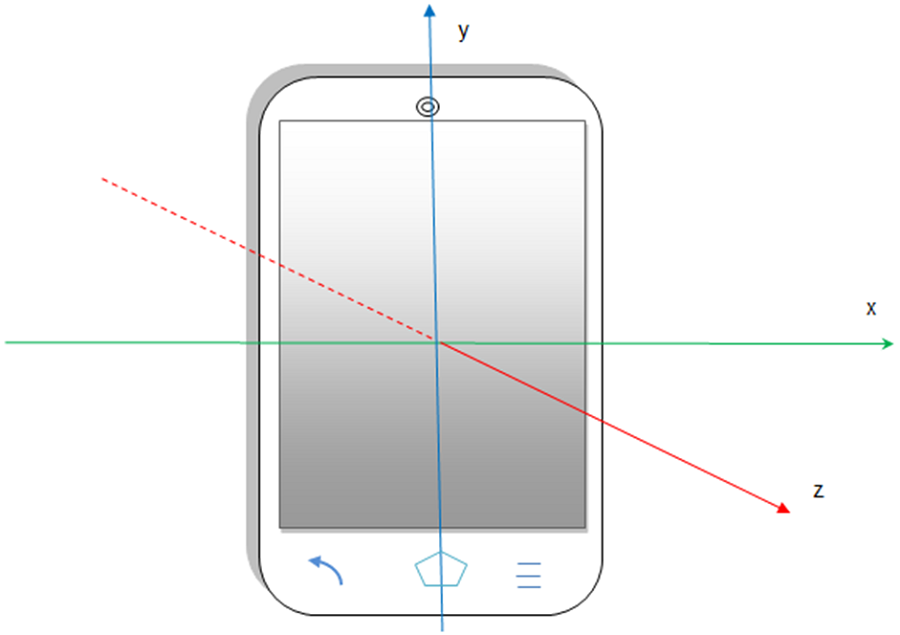
\includegraphics[width=0.3\paperwidth]{img/SensorCoordinateSystemSmartphone}}\hspace{0.05\paperwidth}\subfloat[Sensor coordinate system for tablet]{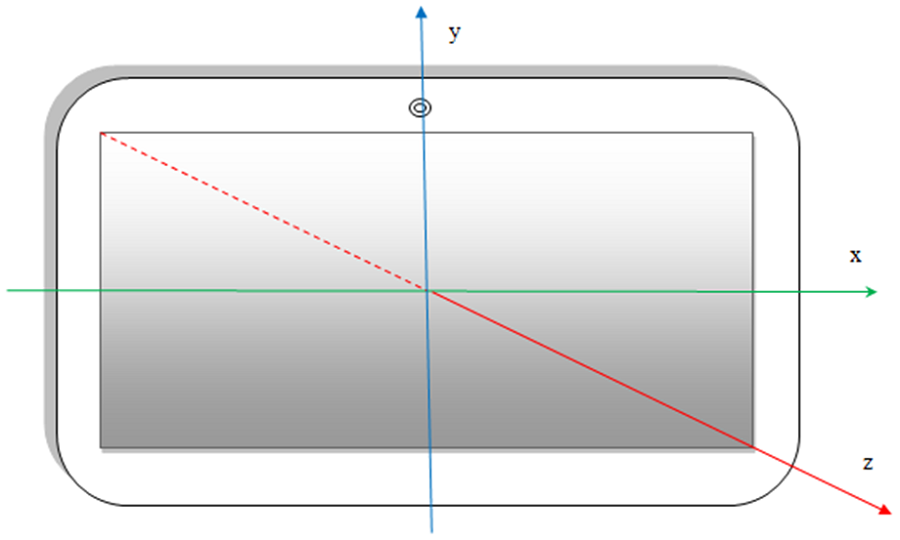
\includegraphics[width=0.3\paperwidth]{img/SensorCoordinateSystemTablet}

}
\end{figure}

\par\end{center}


\subsection{\textcolor{black}{Identifying sensors and sensor capabilities}}

\textcolor{black}{The Android sensor framework provides several methods
that make it easy determine at runtime which sensors are on a device
and the capabilities of each sensor, such as maximum range, resolution,
power requirements, minimum delay and vendor.}

\textcolor{black}{First of all, to identify the sensors on a device,
is necessary to obtain a reference to the sensor service by creating
an instance of the }\texttt{\textcolor{black}{\small{}SensorManager}}\textcolor{black}{{}
class by calling the }\texttt{\textcolor{black}{getSystemService()}}\textcolor{black}{{}
method using the }\texttt{\textcolor{black}{SENSOR\_SERVICE}}\textcolor{black}{{}
as parameter:}

\begin{center}
\textcolor{black}{}%
\ovalbox{\begin{minipage}[c]{0.77\paperwidth}%
\begin{lyxcode}
\textcolor{black}{}
\begin{lstlisting}[basicstyle={\footnotesize\sffamily},comment={[l]{//}},commentstyle={\color{darkgreen}\ttfamily},emph={int, boolean, int, float, double, List,  Sensor, SensorManager, Context},emphstyle={\color{blue}},identifierstyle={\color{black}},keywords={typeof, new, true, false, catch, function, return, null, catch, switch, var, if, in, while, do, else, case, break, int, long, this, new},keywordstyle={\color{magenta}\bfseries},language=Java,morecomment={[s]{/*}{*/}},ndkeywords={class, export, throw, implements, import, this},ndkeywordstyle={\color{darkgray}\bfseries},sensitive=false,stringstyle={\color{red}\ttfamily},tabsize=4]
private SensorManager mSensorManager;
mSensorManager = (SensorManager) getSystemService(Context.SENSOR_SERVICE);
\end{lstlisting}
\end{lyxcode}
%
\end{minipage}}
\par\end{center}

\textcolor{black}{Now, calling the}\texttt{\textbf{\textcolor{black}{{}
}}}\texttt{\textcolor{black}{getSensorList()}}\textcolor{black}{{} method
and using }\texttt{\textcolor{black}{TYPE\_ALL}}\textcolor{black}{{}
constant as parameter, }\texttt{\textcolor{black}{\small{}SensorManager}}\textcolor{black}{{}
returns the list of every sensor on the device:}

\begin{center}
\textcolor{black}{}%
\ovalbox{\begin{minipage}[c]{0.77\paperwidth}%
\begin{lyxcode}
\textcolor{black}{}
\begin{lstlisting}[basicstyle={\footnotesize\sffamily},comment={[l]{//}},commentstyle={\color{darkgreen}\ttfamily},emph={int, boolean, int, float, double, List,  Sensor, SensorManager, Context},emphstyle={\color{blue}},identifierstyle={\color{black}},keywords={typeof, new, true, false, catch, function, return, null, catch, switch, var, if, in, while, do, else, case, break, int, long, this, new},keywordstyle={\color{magenta}\bfseries},language=Java,morecomment={[s]{/*}{*/}},ndkeywords={class, export, throw, implements, import, this},ndkeywordstyle={\color{darkgray}\bfseries},sensitive=false,stringstyle={\color{red}\ttfamily},tabsize=4]
List<Sensor> deviceSensors = mSensorManager.getSensorList(Sensor.TYPE_ALL);
\end{lstlisting}
\end{lyxcode}
%
\end{minipage}}
\par\end{center}

\textcolor{black}{Using, instead of }\texttt{\textcolor{black}{TYPE\_ALL}}\textcolor{black}{{}
constant, another constant provided by }\texttt{\textcolor{black}{\small{}Sensor}}\textcolor{black}{{}
class such as }\texttt{\textcolor{black}{TYPE\_GYROSCOPE}}\textcolor{black}{,
}\texttt{\textcolor{black}{TYPE\_LINEAR\_ACCELERATION}}\textcolor{black}{,
}\texttt{\textcolor{black}{TYPE\_GRAVITY}}\textcolor{black}{{} etc.
}\texttt{\textcolor{black}{\small{}SensorManager}}\textcolor{black}{{}
class returns a lists all sensors of the given type.}

\textcolor{black}{Is also possible determine if a specific type of
sensor exists on a device by using the }\texttt{\textcolor{black}{getDefaultSensor()}}\textcolor{black}{{}
method with the sensor type constant as parameter. If a device has
more then one sensor for the given type, one of its must be designed
as the default sensor and if the default sensor does not exist, the
method returns null (which means that the device does not have thay
type of sensor). The following code checks if there is an accelerometer
on the device:}

\begin{center}
\ovalbox{\begin{minipage}[c]{0.77\paperwidth}%
\begin{lyxcode}
\begin{lstlisting}[basicstyle={\footnotesize\sffamily},comment={[l]{//}},commentstyle={\color{darkgreen}\ttfamily},emph={int, boolean, int, float, double, Sensor, SensorManager, Context},emphstyle={\color{blue}},identifierstyle={\color{black}},keywords={typeof, new, true, false, catch, function, return, null, catch, switch, var, if, in, while, do, else, case, break, int, long, this, new},keywordstyle={\color{magenta}\bfseries},language=Java,morecomment={[s]{/*}{*/}},ndkeywords={class, export, throw, implements, import, this},ndkeywordstyle={\color{darkgray}\bfseries},sensitive=false,stringstyle={\color{red}\ttfamily},tabsize=4]
private SensorManager mSensorManager;
...
mSensorManager = (SensorManager) getSystemService(Context.SENSOR_SERVICE);
if ( mSensorManager.getDefaultSensor(Sensor.TYPE_ACCELEROMETER) != null ) {
	// Success! There's an accelerometer.
}
else{
	// Failure! No accelerometer.
}
\end{lstlisting}
\end{lyxcode}
%
\end{minipage}}
\par\end{center}

\begin{center}

\par\end{center}

In addition to listing the sensors on a device, in possible, using
public methods of Sensor class, determine capabilities and attributes
of each sensor. This is useful if an application can have different
behavior depending on sensors, or sensor capabilities, available on
a device. With this methods is possible to obtain sensor's resolution
and maximum range of measurement (using \texttt{getResolution()} and
\texttt{getMaximumRange()}) or sensor's power requirement with \texttt{getPower()}
method; other two methods particularly useful to optimize an application
for different manufacturers' sensors or different sensors' version
are\texttt{ getVendor()} -for the manufacturer- and \texttt{getVersion()}
-to obtain sensor's version-.

The following sample code shows how to use \texttt{getVendor()} and
\texttt{getVersion()} methods to optimize an application using gravity
sensor if its vendor is \textsl{Google Inc.} and its version is \textsl{3},
if that particular sensor is not present on device the application
try to use the accelerometer:

Another useful methods is the \texttt{getMinDelay()} which returns
the minimum time interval (in microseconds) between two data sensed
by a sensor. Any sensor that returns a \textit{non-zero} value is
a streaming sensor -this type of sensors sense data at regular intervals
and were introduced by Android 2.3 Gingerbread (API Level 9)- while
if a sensor returns zero, it means that the sensor is not streaming
sensor, and it reports data only when there is a chenge in the paremeter
it is sensing. This method is useful because using it in possible
to determine the maximum rate at which a sensor can acquire data.

\newpage{}


\paragraph{Sensors identification code%
\footnote{This app is available on github in AboutSensors project%
}}

The following code realize an Android application that lists all sensors
in a device and its own properties. Some methods were not introduced
until API Level 9, so it works on Android 2.3 (Gingerbread) or latest.

The layout file (\texttt{\textcolor{black}{res/layout/activity\_about\_sensors.xml}})
defines the Android widgets used, their ID and their properties (position,
dimensions, alignment, etc.). In this application is needed a \texttt{\textcolor{black}{Spinner}}
to select which is the sensor to be inspected and a \texttt{\textcolor{black}{TableLayout}}
that contains a row for each property and every row contains two \texttt{\textcolor{black}{TextView}}
(a label and a value field).\\
\\


\ovalbox{\begin{minipage}[t]{1\columnwidth}%
\qquad{}\texttt{\textsl{\textcolor{black}{activity\_about\_sensors.xml}}}

\begin{lstlisting}[basicstyle={\footnotesize\sffamily},breaklines=true,language=XML,lastline=67,tabsize=4]
<?xml version="1.0" encoding="utf-8"?>
<RelativeLayout xmlns:android="http://schemas.android.com/apk/res/android"
    android:layout_width="match_parent"
    android:layout_height="match_parent" >
    <Spinner
        android:id="@+id/spinner_sensors"
        android:layout_width="wrap_content"
        android:layout_height="wrap_content"
        android:layout_alignParentLeft="true"
        android:layout_alignParentTop="true" />
    <TableLayout
        android:layout_width="wrap_content"
        android:layout_height="wrap_content"
        android:layout_alignParentLeft="true"
        android:layout_alignParentRight="true"
        android:layout_below="@+id/spinner_sensors" >
        <TableRow
            android:id="@+id/tableRowVersion"
            android:layout_width="wrap_content"
            android:layout_height="wrap_content" >
            <TextView
               android:id="@+id/labelVersion"
                android:layout_width="wrap_content"
                android:layout_height="wrap_content"
                android:text="Version: "
                android:textAppearance="?android:attr/textAppearanceMedium" />
            <TextView
                android:id="@+id/valueVersion"
                android:layout_width="wrap_content"
                android:layout_height="wrap_content"
                android:text=""
                android:textAppearance="?android:attr/textAppearanceMedium" />
        </TableRow>
        <TableRow
            android:id="@+id/tableRowVendor"
            android:layout_width="wrap_content"
            android:layout_height="wrap_content" >
            <TextView
                android:id="@+id/labelVendor"
                android:layout_width="wrap_content"
                android:layout_height="wrap_content"
                android:text="Vendor: "
                android:textAppearance="?android:attr/textAppearanceMedium" />
            <TextView
                android:id="@+id/valueVendor"
                android:layout_width="wrap_content"
                android:layout_height="wrap_content"
                android:text=""
                android:textAppearance="?android:attr/textAppearanceMedium" />
        </TableRow>
\end{lstlisting}
%
\end{minipage}}

\ovalbox{\begin{minipage}[t]{1\columnwidth}%
\begin{lstlisting}[basicstyle={\footnotesize\sffamily},breaklines=true,language=XML,tabsize=4]
    	<TableRow
            android:id="@+id/tableRowPower"
            android:layout_width="wrap_content"
            android:layout_height="wrap_content" >
            <TextView
                android:id="@+id/labelPower"
                android:layout_width="wrap_content"
                android:layout_height="wrap_content"
                android:text="Power: "
                android:textAppearance="?android:attr/textAppearanceMedium" />
            <TextView
                android:id="@+id/valuePower"
                android:layout_width="wrap_content"
                android:layout_height="wrap_content"
                android:text=""
                android:textAppearance="?android:attr/textAppearanceMedium" />
        </TableRow>    
		<TableRow
            android:id="@+id/tableRowMaxRange"
            android:layout_width="wrap_content"
            android:layout_height="wrap_content" >
            <TextView
                android:id="@+id/labelMaxRange"
                android:layout_width="wrap_content"
                android:layout_height="wrap_content"
                android:text="Maximum Range: "
                android:textAppearance="?android:attr/textAppearanceMedium" />
            <TextView
                android:id="@+id/valueMaxRange"
                android:layout_width="wrap_content"
                android:layout_height="wrap_content"
                android:text=""
                android:textAppearance="?android:attr/textAppearanceMedium" />
        </TableRow>
        <TableRow
            android:id="@+id/tableRowResolution"
            android:layout_width="wrap_content"
            android:layout_height="wrap_content" >
            <TextView
                android:id="@+id/labelResolution"
                android:layout_width="wrap_content"
                android:layout_height="wrap_content"
                android:text="Resolution: "
                android:textAppearance="?android:attr/textAppearanceMedium" />
            <TextView
                android:id="@+id/valueResolution"
                android:layout_width="wrap_content"
                android:layout_height="wrap_content"
                android:text=""
                android:textAppearance="?android:attr/textAppearanceMedium" />
        </TableRow>
        <TableRow
            android:id="@+id/tableRowMinDelay"
            android:layout_width="wrap_content"
            android:layout_height="wrap_content" >
            <TextView
                android:id="@+id/labelMinDelay"
                android:layout_width="wrap_content"
                android:layout_height="wrap_content"
                android:text="Minimum Delay: "
                android:textAppearance="?android:attr/textAppearanceMedium" />
            <TextView
                android:id="@+id/valueMinDelay"
                android:layout_width="wrap_content"
                android:layout_height="wrap_content"
                android:text=""
                android:textAppearance="?android:attr/textAppearanceMedium" />
        </TableRow>
   </TableLayout>
</RelativeLayout> 
\end{lstlisting}
%
\end{minipage}}

~

The activity code is really simple: when Android system creates the
activity (\texttt{onCreate()} method), the first thing to do is the
initialization of resources. The \texttt{initializeResources()} method
assigns to each field its resource referenced in layout file, creates
the \texttt{Spinner}'s \texttt{ArrayAdapter} with sensors' names and
call the \texttt{addSpinnerListener()} method that assigns to the
\texttt{Spinner} a new \texttt{onItemSelectedListener} that changes
the shown values with the sensor selected values.\\


\ovalbox{\begin{minipage}[t]{1\columnwidth}%
\qquad{}\texttt{\textsl{\textcolor{black}{AboutSensors.java}}}

\begin{lstlisting}[basicstyle={\footnotesize\ttfamily},breaklines=true,comment={[l]{//}},commentstyle={\color{darkgreen}\ttfamily},emph={int, boolean, int, float, double, List,  Sensor, SensorManager, Context, Bundle, ArrayList, Activity, View, AdapterView, OnItemSelectedListener, ArrayAdapter, Spinner, TextView},emphstyle={\color{blue}},identifierstyle={\color{black}},keywords={typeof, new, true, false, catch, function, return, null, catch, switch, var, if, in, while, do, else, case, break, int, long, this, new},keywordstyle={\color{magenta}\bfseries},language=Java,lastline=67,morecomment={[s]{/*}{*/}},ndkeywords={class, export, @Override},ndkeywordstyle={\color{gray}\bfseries},sensitive=false,stringstyle={\color{red}\ttfamily},tabsize=4]
package it.unibo.android.aboutSensors;

import java.util.ArrayList;
import java.util.List;

import android.app.Activity;
import android.hardware.Sensor;
import android.hardware.SensorManager;
import android.os.Bundle;
import android.view.View;
import android.widget.AdapterView;
import android.widget.AdapterView.OnItemSelectedListener;
import android.widget.ArrayAdapter;
import android.widget.Spinner;
import android.widget.TextView;

public class AboutSensors extends Activity {

	//fields definition
	private Spinner spinnerList;
	private SensorManager manager;
	private List<Sensor> sensors;
	private Sensor sensorSelected;
	private ArrayAdapter<String> adapter;
	private TextView textVersion;
	private TextView textVendor;
	private TextView textPower;
	private TextView textMaxRange;
	private TextView textResolution;
	private TextView textMinDelay;

	@Override
	protected void onCreate(Bundle savedInstanceState) {
		super.onCreate(savedInstanceState);
		//set the default layout
		setContentView(R.layout.activity_about_sensors);
		//initialize the resources
		initializeResources();
	}

	private void initializeResources() {
		//obtain the SensorManager instance and get the sensors list
		manager = (SensorManager) getSystemService(SENSOR_SERVICE);
		sensors = manager.getSensorList(Sensor.TYPE_ALL);
		//get the TextView where put the sensor information
		textVersion = (TextView)findViewById(R.id.valueVersion);
		textVendor = (TextView)findViewById(R.id.valueVendor);
		textPower = (TextView)findViewById(R.id.valuePower);
		textMaxRange = (TextView)findViewById(R.id.valueMaxRange);
		textResolution = (TextView)findViewById(R.id.valueResolution);
		textMinDelay = (TextView)findViewById(R.id.valueMinDelay);
		//get the spinner
		spinnerList = (Spinner)findViewById(R.id.spinner_sensors);
		//set up the spinner adapter with sensors names
		adapter = new ArrayAdapter<String>(this, android.R.layout.simple_spinner_item, 
											getSensorsNames());
		adapter.setDropDownViewResource(android.R.layout.simple_dropdown_item_1line);
		spinnerList.setAdapter(adapter);
		//add the spinner listener
		addSpinnerListener(); 		
	}
\end{lstlisting}
%
\end{minipage}}

\ovalbox{\begin{minipage}[t]{1\columnwidth}%
\begin{lstlisting}[basicstyle={\footnotesize\ttfamily},breaklines=true,comment={[l]{//}},commentstyle={\color{darkgreen}\ttfamily},emph={int, boolean, int, float, double, List,  Sensor, SensorManager, Context, Bundle, ArrayList, Activity, View, AdapterView, OnItemSelectedListener, ArrayAdapter, Spinner, TextView},emphstyle={\color{blue}},identifierstyle={\color{black}},keywords={typeof, new, true, false, catch, function, return, null, catch, switch, var, if, in, while, do, else, case, break, int, long, this, new},keywordstyle={\color{magenta}\bfseries},language=Java,lastline=67,morecomment={[s]{/*}{*/}},ndkeywords={class, export, @override},ndkeywordstyle={\color{gray}\bfseries},sensitive=false,stringstyle={\color{red}\ttfamily},tabsize=4]
	private void addSpinnerListener() {
		spinnerList.setOnItemSelectedListener(new OnItemSelectedListener(){

		@Override
			public void onItemSelected(AdapterView<?> parent, View view, 
										int position, long id) {
				//when an item is selected update the text view 
				//with the selected sensor's informations
				Sensor s = sensors.get(position);
				if(s != sensorSelected){
					System.out.println(s.toString());
					textVersion.setText(""+s.getVersion());
					textVendor.setText(""+s.getVendor());
					textPower.setText(s.getPower()+" mA");
					textMaxRange.setText(""+s.getMaximumRange());
					textResolution.setText(""+s.getResolution());
					textMinDelay.setText(s.getMinDelay()/1000+" ms");
					sensorSelected = s;
				}
			}

			@Override
			public void onNothingSelected(AdapterView<?> parent) {
				textVersion.setText(""); 
				textVendor.setText("");
			}		
		});
	}

	private List<String> getSensorsNames() {
		//returns the list that contains the names of all available sensors
		List<String> sensorNames = new ArrayList<String>();
		for (Sensor s: sensors)
			sensorNames.add(s.getName());
		return sensorNames;
	} 
}
\end{lstlisting}
%
\end{minipage}}


\subsection{Monitoring sensor events}

SensorEventListener interface introduces two callback methods which
must be implemented to monitor raw sensor data. This methods are \texttt{onAccuracyChanged()}
and \texttt{onSensorChanged()}.

This two methods are invoked by Android system, the first whenever
the sensor's accuracy changes (this method provides the reference
to the \texttt{Sensor} object that changed and its new accuracy, whose
state is represented by one of four constants defined in \texttt{SensorManager}
class:
\begin{itemize}
\item \texttt{SENSOR\_STATUS\_ACCURACY\_LOW}
\item \texttt{SENSOR\_STATUS\_ACCURACY\_MEDIUM}
\item \texttt{SENSOR\_STATUS\_ACCURACY\_HIGH}
\item \texttt{SENSOR\_STATUS\_ACCURACY\_UNRELIABLE}
\end{itemize}
The \texttt{onSensorChanged()} method, insted, is invoked by system
when a sensor reports a new value. This method provides a new \texttt{SensorEvent}
object that contains informations about the new sensor data (the new
data recorded by the sensor, its accuracy, the sensor which generates
the new data and the relative timestamp).


\paragraph{Sensor events code%
\footnote{This app is available on github in the project AboutSensorEvents%
}}

The following code is based on AboutSensors project. In this application
is shown, with the previous informations, the raw sensor data, received
by the selected sensor.

In layout file (\texttt{\textcolor{black}{res/layout/activity\_about\_sensor\_events.xml}})
above the sensor informations table is defined a new table that contains
3 rows with 3 labels and 3 \texttt{TextView}, one for each axes value
(X, Y and Z). The following code shown only the difference between
the previous and the new layout. 

This part of code begins after the \lstinline[basicstyle={\small\ttfamily},language=XML]!</TableLayout>!
tag.

\ovalbox{\begin{minipage}[t]{1\columnwidth}%
\qquad{}\texttt{\textsl{\textcolor{black}{activity\_about\_sensor\_events.xml}}}

\begin{lstlisting}[basicstyle={\footnotesize\sffamily},breaklines=true,language=XML,lastline=67,tabsize=4]
    <TextView
        android:id="@+id/LabelSensorData"
        android:layout_width="wrap_content"
        android:layout_height="wrap_content"
        android:layout_alignParentLeft="false"
        android:layout_alignParentRight="false"
        android:layout_below="@+id/tableLayout1"
        android:layout_centerHorizontal="true"
        android:text="Sensor Data:"
        android:textAppearance="?android:attr/textAppearanceLarge" />
    <TableLayout
        android:id="@+id/SensorData"
        android:layout_width="wrap_content"
        android:layout_height="wrap_content"
        android:layout_alignParentLeft="true"
        android:layout_alignParentRight="true"
        android:layout_below="@+id/LabelSensorData" >
        <TableRow
            android:id="@+id/SensorDataX"
            android:layout_width="wrap_content" 
            android:layout_height="wrap_content" >
            <TextView
                android:id="@+id/LabelDataX"
                android:layout_width="wrap_content"
                android:layout_height="wrap_content"
                android:text="SensorDataX: "
                android:textAppearance="?android:attr/textAppearanceMedium" />
            <TextView
                android:id="@+id/ValueDataX"
                android:layout_width="wrap_content"
                android:layout_height="wrap_content"
                android:textAppearance="?android:attr/textAppearanceMedium" />
        </TableRow>
		<TableRow
            android:id="@+id/SensorDataY"
            android:layout_width="wrap_content" 
            android:layout_height="wrap_content" >
            <TextView
                android:id="@+id/LabelDataY"
                android:layout_width="wrap_content"
                android:layout_height="wrap_content"
                android:text="SensorDataY: "
                android:textAppearance="?android:attr/textAppearanceMedium" />
            <TextView
                android:id="@+id/ValueDataY"
                android:layout_width="wrap_content"
                android:layout_height="wrap_content"
                android:textAppearance="?android:attr/textAppearanceMedium" />
        </TableRow>
		<TableRow
            android:id="@+id/SensorDataZ"
            android:layout_width="wrap_content" 
            android:layout_height="wrap_content" >
            <TextView
                android:id="@+id/LabelDataZ"
                android:layout_width="wrap_content"
                android:layout_height="wrap_content"
                android:text="SensorDataZ: "
                android:textAppearance="?android:attr/textAppearanceMedium" />
            <TextView
                android:id="@+id/ValueDataZ"
                android:layout_width="wrap_content"
                android:layout_height="wrap_content"
                android:textAppearance="?android:attr/textAppearanceMedium" />
        </TableRow>
	</TableLayout>
</RelativeLayout>
\end{lstlisting}
%
\end{minipage}}\newpage{}The activity, like the \texttt{AboutSensor} application,
changes sensors information when a new sensor is selected from \texttt{Spinner}
and shows, in addition to sensor informations, the sensor row data
updated by the sensor event listener, in fact, the \texttt{SpinnerListener},
by \texttt{onItemSelected} method, changes the \texttt{SensorEventsListener}
calling the \texttt{updateSensorListener} method, which removes old
listener from previous selected sensor and attaches to the new selected
sensor a new listener. This method is called too when the application
is resumed (\texttt{onResume()} method), and, when the application
is paused (\texttt{onPause()} method) the sensor listener is detached
from sensor.

The \texttt{SensorEventsListener} class extends \texttt{SensorEventListener}
interface the defines
\begin{itemize}
\item \texttt{onSensorChanged} method that updates the sensor data's text
views
\item \texttt{onAccuracyChanged} that, in this case, does nothing
\end{itemize}
~

\ovalbox{\begin{minipage}[t]{1\columnwidth}%
\qquad{}\texttt{\textsl{\textcolor{black}{AboutSensorEvents.java}}}

\begin{lstlisting}[basicstyle={\footnotesize\ttfamily},breaklines=true,comment={[l]{//}},commentstyle={\color{darkgreen}\ttfamily},emph={int, boolean, int, float, double, List,  Sensor, SensorManager, Context, Bundle, ArrayList, Activity, View, AdapterView, OnItemSelectedListener, ArrayAdapter, Spinner, TextView},emphstyle={\color{blue}},identifierstyle={\color{black}},keywords={typeof, new, true, false, catch, function, return, null, catch, switch, var, if, in, while, do, else, case, break, int, long, this, new},keywordstyle={\color{magenta}\bfseries},language=Java,lastline=67,morecomment={[s]{/*}{*/}},ndkeywords={class, export, @Override},ndkeywordstyle={\color{gray}\bfseries},sensitive=false,stringstyle={\color{red}\ttfamily},tabsize=4]
package it.unibo.android.aboutSensorEvents;

import java.util.ArrayList;
import java.util.List;

import android.app.Activity;
import android.hardware.Sensor;
import android.hardware.SensorEvent;
import android.hardware.SensorEventListener;
import android.hardware.SensorManager;
import android.os.Bundle;
import android.view.View;
import android.widget.AdapterView;
import android.widget.AdapterView.OnItemSelectedListener;
import android.widget.ArrayAdapter;
import android.widget.Spinner;
import android.widget.TextView;

public class AboutSensorEvents extends Activity {
	//fields definition
	private Spinner spinnerList;
	private SensorManager manager;
	private List<Sensor> sensors;
	private Sensor sensorSelected;
	private ArrayAdapter<String> adapter;
	private TextView textVersion;
	private TextView textVendor;
	private TextView textPower;
	private TextView textMaxRange;
	private TextView textResolution;
	private TextView textMinDelay;
	private SensorEventListener listener;
	private TextView textX;
	private TextView textY;
	private TextView textZ;

	@Override
	protected void onCreate(Bundle savedInstanceState) {
		super.onCreate(savedInstanceState);
		//set the default layout
		setContentView(R.layout.activity_about_sensor_events);
		//initialize the resources
		initializeResources();
	}

	@Override
	protected void onResume() {
		super.onResume();
		manager.registerListener(listener, sensorSelected, SensorManager.SENSOR_DELAY_NORMAL);
	}

	@Override
	protected void onPause() {
		super.onPause();
		manager.unregisterListener(listener, sensorSelected);
	}
\end{lstlisting}
%
\end{minipage}}

\ovalbox{\begin{minipage}[t]{1\columnwidth}%
\begin{lstlisting}[basicstyle={\footnotesize\ttfamily},breaklines=true,comment={[l]{//}},commentstyle={\color{darkgreen}\ttfamily},emph={int, boolean, int, float, double, List,  Sensor, SensorManager, Context, Bundle, ArrayList, Activity, View, AdapterView, OnItemSelectedListener, ArrayAdapter, Spinner, TextView},emphstyle={\color{blue}},identifierstyle={\color{black}},keywords={typeof, new, true, false, catch, function, return, null, catch, switch, var, if, in, while, do, else, case, break, int, long, this, new},keywordstyle={\color{magenta}\bfseries},language=Java,lastline=67,morecomment={[s]{/*}{*/}},ndkeywords={class, export, @override},ndkeywordstyle={\color{gray}\bfseries},sensitive=false,stringstyle={\color{red}\ttfamily},tabsize=4]
	private void initializeResources() {
		//obtain the SensorManager instance and get the sensors list
		manager = (SensorManager) getSystemService(SENSOR_SERVICE);
		sensors = manager.getSensorList(Sensor.TYPE_ALL);
		//get the TextView where put the sensor information
		textVersion = (TextView)findViewById(R.id.valueVersion);
		textVendor = (TextView)findViewById(R.id.valueVendor);
		textPower = (TextView)findViewById(R.id.valuePower);
		textMaxRange = (TextView)findViewById(R.id.valueMaxRange);
		textResolution = (TextView)findViewById(R.id.valueResolution);
		textMinDelay = (TextView)findViewById(R.id.valueMinDelay);
		//get the TextView where put sensor raw data received
		textX = (TextView)findViewById(R.id.ValueDataX);
		textY = (TextView)findViewById(R.id.ValueDataY);
		textZ = (TextView)findViewById(R.id.ValueDataZ);
		//get the spinner
		spinnerList = (Spinner)findViewById(R.id.spinner_sensors);
		//set up the spinner adapter with sensors names
		adapter = new ArrayAdapter<String>(this, android.R.layout.simple_spinner_item,
											getSensorsNames());
		adapter.setDropDownViewResource(android.R.layout.simple_dropdown_item_1line);
		spinnerList.setAdapter(adapter);
		//add the spinner listener
		addSpinnerListener();
	}

	private void updateSensorListener() {
		//if exist a defined listener remove it from sensor
		if(listener!=null)
			manager.unregisterListener(listener, sensorSelected);
		//register new listener
		listener = new SensorEventsListener();
		manager.registerListener(listener,
								sensors.get(spinnerList.getSelectedItemPosition()),
								SensorManager.SENSOR_DELAY_NORMAL);
	}

	private void addSpinnerListener() {
		spinnerList.setOnItemSelectedListener(new OnItemSelectedListener(){

		@Override
			public void onItemSelected(AdapterView<?> parent, View view, 
										int position, long id) {
				//when an item is selected update the text view 
				//with the selected sensor's informations
				Sensor s = sensors.get(position);
				if(s != sensorSelected){
					System.out.println(s.toString());
					textVersion.setText(""+s.getVersion());
					textVendor.setText(""+s.getVendor());
					textPower.setText(s.getPower()+" mA");
					textMaxRange.setText(""+s.getMaximumRange());
					textResolution.setText(""+s.getResolution());
					textMinDelay.setText(s.getMinDelay()/1000+" ms");
					updateSensorListener();
					sensorSelected = s;
				}
			}

			@Override
			public void onNothingSelected(AdapterView<?> parent) {
				textVersion.setText(""); 
				textVendor.setText("");
			}		
		});
	}
\end{lstlisting}
%
\end{minipage}}

\ovalbox{\begin{minipage}[t]{1\columnwidth}%
\begin{lstlisting}[basicstyle={\footnotesize\ttfamily},breaklines=true,comment={[l]{//}},commentstyle={\color{darkgreen}\ttfamily},emph={int, boolean, int, float, double, List,  Sensor, SensorManager, Context, Bundle, ArrayList, Activity, View, AdapterView, OnItemSelectedListener, ArrayAdapter, Spinner, TextView},emphstyle={\color{blue}},identifierstyle={\color{black}},keywords={typeof, new, true, false, catch, function, return, null, catch, switch, var, if, in, while, do, else, case, break, int, long, this, new},keywordstyle={\color{magenta}\bfseries},language=Java,lastline=67,morecomment={[s]{/*}{*/}},ndkeywords={class, export, @override},ndkeywordstyle={\color{gray}\bfseries},sensitive=false,stringstyle={\color{red}\ttfamily},tabsize=4]
	private List<String> getSensorsNames() {
		//returns the list that contains the names of all available sensors
		List<String> sensorNames = new ArrayList<String>();
		for (Sensor s: sensors)
			sensorNames.add(s.getName());
		return sensorNames;
	} 

	private class SensorEventsListener implements SensorEventListener {

		@Override
		public void onSensorChanged(SensorEvent event) {
			//show values
			textX.setText(""+event.values[0]);
			textY.setText(""+event.values[1]);
			textZ.setText(""+event.values[2]);
		}

		@Override
		public void onAccuracyChanged(Sensor sensor, int accuracy) {
			//do something when accuracy changes
		}
	}
}
\end{lstlisting}
%
\end{minipage}}


\subsection{Best practices for accessing and using sensors}

In this section are discussed the guidelines to design an optimized
sensor implementation. 

These guidelines are recommended best practices for anyone who is
using the sensor framework to access sensors and acquire sensor data.


\subsubsection*{Verify sensors' availability}

Android platform does not require to the manufacturer that a device
includes particular sensors, then, before using a specific sensor
it is necessary to check if this sensor exists. 

Assume the existence of a sensor simply because is frequently used
is a bad practice.


\subsubsection*{Unregister sensor listeners}

If a sensor listener is registered and its activity is paused, the
sensor will continue to acquire data and use battery resources unless
the listener is unregisterd. The bettter way to optimize resources
usage is to unregister the listener each time the application is paused,
or the sensor is no longer needed, and then register it again when
the app is resumed. This is possible using two methods provided by
the \texttt{Activity} class:
\begin{description}
\item [{\texttt{onPause()}}] called when the application is going down
(or lost the screen)
\item [{\texttt{onResume()}}] invoked when the application comes back to
the screen
\end{description}
The following code is an example that show how to use this two methods
in an \texttt{Activity} that implements \texttt{SensorEventListener}
interface:

\begin{center}
\textcolor{black}{}%
\ovalbox{\begin{minipage}[c]{0.77\paperwidth}%
\begin{lyxcode}
\textcolor{black}{}
\begin{lstlisting}[basicstyle={\footnotesize\sffamily},comment={[l]{//}},commentstyle={\color{darkgreen}\ttfamily},emph={int, boolean, int, float, double, List,  Sensor, SensorManager, Context, Bundle, ArrayList, Activity, View, AdapterView, OnItemSelectedListener, ArrayAdapter, Spinner, TextView},emphstyle={\color{blue}},identifierstyle={\color{black}},keywords={typeof, new, true, false, catch, function, return, null, catch, switch, var, if, in, while, do, else, case, break, int, long, this, new},keywordstyle={\color{magenta}\bfseries},language=Java,morecomment={[s]{/*}{*/}},ndkeywords={class, export, @Override},ndkeywordstyle={\color{gray}\bfseries},sensitive=false,stringstyle={\color{red}\ttfamily},tabsize=4]
private SensorManager mSensorManager;
private Sensor mSensor
  ... 

@Override protected void onPause() {
  super.onPause();
  mSensorManager.unregisterListener(this, mSensor);
}

@Override protected void onResume() {
  super.onResume();
  mSensorManager.registerListener(this, mSensor, SensorManager.SENSOR_DELAY_NORMAL);
}
\end{lstlisting}
\end{lyxcode}
%
\end{minipage}}
\par\end{center}


\subsubsection*{Don't test your code on the emulator}

The Android emulator cannot emulate sensors, thus, currently, is not
possible to test the sensor code on Android Virtual Devices. The best
way to run a test on sensor code is by using a physical device. There
are, however, sensor simulators that can be used to simulate sensor
output.


\subsubsection*{Don't block the onSensorChanged() method}

Android system may call the \texttt{onSensorChanged(SensorEvent)}
method quite often because sensor data can changes at high rate, hence
is recommended, as the best practice, do as little is possible into
\texttt{onSensorChanged(SensorEvent)} so as not to block his execution.

If an application requires any data filtering or reduction of sensor
data, it would be better perform that work outside of the \texttt{onSensorChanged(SensorEvent)}
method.


\subsubsection*{Avoid using deprecated methods or sensor types}

Several methods and constants, such as \texttt{TYPE\_ORIENTATION}
or \texttt{TYPE\_TEMPERATURE}, have been deprecated, the first has
been replaced by \texttt{getOrientation()} method and the second,
in devices that are running Android 4 Ice Cream Sandwich, by \texttt{TYPE\_AMBIENT\_TEMPERATURE}
constant.


\subsubsection*{Choose sensor delay carefully}

The registerListener() method requires, in addiction to the listener
and the sensor, the minimum delay between two notifications. The choise
of the delivery rate must be suitable for the application or use-case:
sensors can provide data at very high rates and allowing the system
to send extra data which is not needed wastes system resources and
uses battery power. Like the accuracy, Android provides, in SensorManager
class, four differents constants that defines four different delivery
rate:
\begin{description}
\item [{\texttt{SENSOR\_DELAY\_NORMAL}}] delivery rate of 200000\textgreek{m}s 
\item [{\texttt{SENSOR\_DELAY\_UI}}] delivery rate of 60000\textgreek{m}s 
\item [{\texttt{SENSOR\_DELAY\_GAME}}] delivery rate of 20000\textgreek{m}s
\item [{\texttt{SENSOR\_DELAY\_FASTEST}}] delivery rate of 0\textgreek{m}s
(enable the real delay time of the sensor, obtained by \texttt{getMinDelay()}
method)\clearpage{}
\end{description}

\section{Hardware Abstraction Layer for Android sensors}

As mentioned Android sensor framework contains also the SensorHAL
library which provides to manufacturers the links by kernel-space
drivers to the Android sensor service and Android sensor manager.

The image below shows the sensor subsystem, that can be divided in
5 linked layers that allows application to obtain sensors data:

\begin{center}
\begin{figure}[H]
\caption{Android sensor subsystem\cite{sensorHAL}}


\centering{}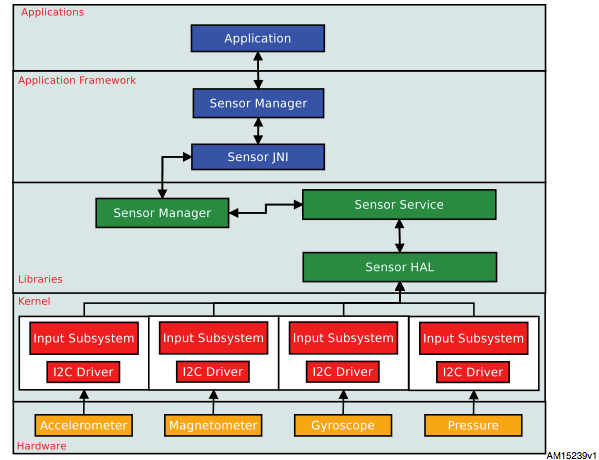
\includegraphics[width=0.45\paperwidth]{img/SensorFramework}
\end{figure}

\par\end{center}
\begin{description}
\item [{Application~Framework}] provides to all application that needs
sensors' informations to get data from device. The communication between
the application and the hardware sensor starts with in \texttt{SensorManager}
class, and, trhough the \texttt{SensorJNI} (Java Native Interface)
pass to the lower layer.
\item [{Sensor~Libraries}] creates a sophisticated interface for the upper
layer using \texttt{SensorManager}, \texttt{SensorService} and \texttt{SensorHAL}
classes
\item [{Kernel}] in this layer are presents Linux device drivers, created
using input subsystem: like a keyboard or a mouse sensor data are
exported to the user space through the sysfs virtual file system (\texttt{/sys/class/input/})
and the driver sends/receives data to/from the sensor through the
Linux subsystem I2C.
\end{description}
A simple way to integrate sensors in Android system, like STMicroelectronics
suggests\cite{sensorHAL}, needs two configuration files one sets
conversion values and the other defines sensors' parameters and informations.
A second and easier way for Android device developers to configure
and enable access to the built-in hardware sensor components of their
devices is DASH\cite{SonyDASH} (Dynamic Android Sensor HAL), developed
by Sony\textsuperscript{\textregistered{}}. Initially this project
was used for Xperia\textsuperscript{\textregistered{}} models, then,
since June 2012, is available on GitHub%
\footnote{Sony DASH repository available at \href{https://github.com/sonyxperiadev/DASH}{https://github.com/sonyxperiadev/DASH}
with Apache License, Version 2.0%
}. With this framework developers can use the same code in different
devices and DASH dynamically configures which sensors are available
at runtime and allows sensor code to call on the sensor's own calibration
libraries and configuration files. DASH makes Sensor HAL framework
generic, configurable and scalable, and also has the advantage of
being open source.

\begin{center}
\begin{figure}[H]
\caption{DASH Framework architecture\cite{AnderoDASHpresentation}}


\centering{}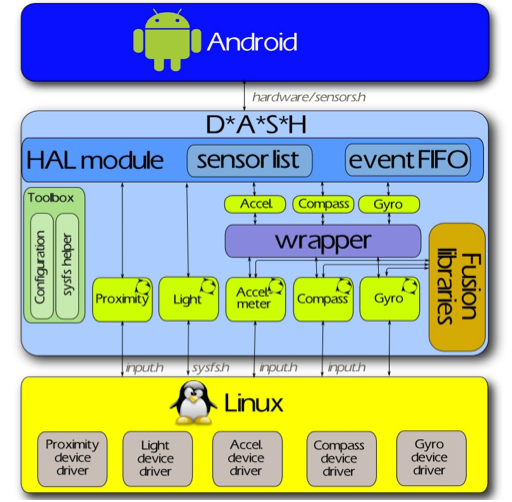
\includegraphics[width=0.45\paperwidth]{img/dash}
\end{figure}

\par\end{center}


\section{Motion Sensors}

\begin{center}
\begin{table}[H]
\caption{Motion sensors available on the Android platform}


\centering{}%
\begin{tabular}{|>{\raggedright}m{0.25\columnwidth}|>{\raggedright}m{0.25\textwidth}|>{\raggedright}m{0.25\textwidth}|>{\raggedright}b{0.1\textwidth}|}
\hline 
\rowcolor{cyan}
\centering\textbf{Sensor} & \centering\texttt{\textbf{SensorEvent}}\textbf{ data} & \centering\textbf{Description} & \centering\textbf{Units of measure}\tabularnewline
\hline 
\hline 
\multirow{3}{0.25\columnwidth}{\texttt{\footnotesize{}TYPE\_ACCELEROMETER}} & \texttt{SensorEvent.values{[}0{]}} & {\small{}Acceleration force along the x axis (including gravity)} & \multirow{3}{0.1\textwidth}{{\small{}
\[
\nicefrac{m}{s^{2}}
\]
}}\tabularnewline
\cline{2-3} 
 & \texttt{SensorEvent.values{[}1{]}} & {\small{}Acceleration force along the y axis (including gravity)} & \tabularnewline
\cline{2-3} 
 & \texttt{SensorEvent.values{[}2{]}} & {\small{}Acceleration force along the z axis (including gravity)} & \tabularnewline
\hline 
\multirow{3}{0.25\columnwidth}{\texttt{\footnotesize{}TYPE\_GRAVITY}} & \texttt{SensorEvent.values{[}0{]}} & {\small{}Force of gravity along the x axis} & \multirow{3}{0.1\textwidth}{{\small{}
\[
\nicefrac{m}{s^{2}}
\]
}}\tabularnewline
\cline{2-3} 
 & \texttt{SensorEvent.values{[}1{]}} & {\small{}Force of gravity along the y axis} & \tabularnewline
\cline{2-3} 
 & \texttt{SensorEvent.values{[}2{]}} & {\small{}Force of gravity along the z axis} & \tabularnewline
\hline 
\multirow{3}{0.25\columnwidth}{\texttt{\footnotesize{}TYPE\_GYROSCOPE}} & \texttt{SensorEvent.values{[}0{]}} & {\small{}Rate of rotation around the x axis} & \multirow{3}{0.1\textwidth}{{\small{}
\[
\nicefrac{rad}{s}
\]
}}\tabularnewline
\cline{2-3} 
 & \texttt{SensorEvent.values{[}1{]}} & {\small{}Rate of rotation around the y axis} & \tabularnewline
\cline{2-3} 
 & \texttt{SensorEvent.values{[}2{]}} & {\small{}Rate of rotation around the z axis} & \tabularnewline
\hline 
\multirow{6}{0.25\columnwidth}{\texttt{\footnotesize{}TYPE\_GYROSCOPE\_UNCALIBRATED}} & \texttt{SensorEvent.values{[}0{]}} & {\small{}Rate of rotation (without drift compensation) around the
x axis} & \multirow{6}{0.1\textwidth}{{\small{}
\[
\nicefrac{rad}{s}
\]
}}\tabularnewline
\cline{2-3} 
 & \texttt{SensorEvent.values{[}1{]}} & {\small{}Rate of rotation (without drift compensation) around the
y axis} & \tabularnewline
\cline{2-3} 
 & \texttt{SensorEvent.values{[}2{]}} & {\small{}Rate of rotation (without drift compensation) around the
z axis} & \tabularnewline
\cline{2-3} 
 & \texttt{SensorEvent.values{[}3{]}} & {\small{}Estimated drift around the x axis} & \tabularnewline
\cline{2-3} 
 & \texttt{SensorEvent.values{[}4{]}} & {\small{}Estimated drift around the y axis} & \tabularnewline
\cline{2-3} 
 & \texttt{SensorEvent.values{[}5{]}} & {\small{}Estimated drift around the z axis} & \tabularnewline
\hline 
\multirow{3}{0.25\columnwidth}{\texttt{\footnotesize{}TYPE\_LINEAR\_ACCELERATION}} & \texttt{SensorEvent.values{[}0{]}} & {\small{}Acceleration force along the x axis (excluding gravity)} & \multirow{3}{0.1\textwidth}{{\small{}
\[
\nicefrac{m}{s^{2}}
\]
}}\tabularnewline
\cline{2-3} 
 & \texttt{SensorEvent.values{[}1{]}} & {\small{}Acceleration force along the y axis (excluding gravity)} & \tabularnewline
\cline{2-3} 
 & \texttt{SensorEvent.values{[}2{]}} & {\small{}Acceleration force along the z axis (excluding gravity)} & \tabularnewline
\hline 
\multirow{4}{0.25\columnwidth}{\texttt{\footnotesize{}TYPE\_ROTATION\_VECTOR}} & \texttt{SensorEvent.values{[}0{]}} & {\small{}Rotation vector component along the x axis ($x*\sin(\theta/2)$)} & \multirow{4}{0.1\textwidth}{{\small{}Unitless}}\tabularnewline
\cline{2-3} 
 & \texttt{SensorEvent.values{[}1{]}} & {\small{}Rotation vector component along the x axis ($y*\sin(\theta/2)$)} & \tabularnewline
\cline{2-3} 
 & \texttt{SensorEvent.values{[}2{]}} & {\small{}Rotation vector component along the x axis ($z*\sin(\theta/2)$)} & \tabularnewline
\cline{2-3} 
 & \texttt{SensorEvent.values{[}3{]}} & {\small{}Optional: scalar component of the rotation vector ($\cos(\theta/2)$)} & \tabularnewline
\hline 
\multirow{1}{0.25\columnwidth}{\texttt{\footnotesize{}TYPE\_SIGNIFICANT\_MOTION}} & {\footnotesize{}N/A} & {\small{}N/A} & \multirow{1}{0.1\textwidth}{{\small{}N/A}}\tabularnewline
\hline 
\multirow{1}{0.25\columnwidth}{\texttt{\footnotesize{}TYPE\_STEP\_COUNTER}} & \texttt{SensorEvent.values{[}0{]}} & {\small{}Number of steps taken by the user since the last reboot while
the sensor was acrivated} & \multirow{1}{0.1\textwidth}{{\small{}Steps}}\tabularnewline
\hline 
\multirow{1}{0.25\columnwidth}{\texttt{\footnotesize{}TYPE\_STEP\_DETECTOR}} & {\footnotesize{}N/A} & {\small{}N/A} & \multirow{1}{0.1\textwidth}{{\small{}N/A}}\tabularnewline
\hline 
\end{tabular}
\end{table}

\par\end{center}

Android platform provides several sensors useful for monitoritoring
device movement such as tilt, shake, rotation or swing. Each movement
is usually a reflection of direct user input (e.g. steering a car
or controlling a ball in games) but it can also be a reflection of
the physical environment in which the device is sitting (e.g. sensor
values changes while the device is moving in a car). In the first
case the sensors' monitoring is relative to the device's frame of
reference, while in the second case the monitoring is relative to
the world's frame of reference, but motion sensors, by themselves,
are not typically used to monitor the device's position, however they
can be used with other sensors to determine the device's position
relative to the world's frame of reference (see \hyperref[sec:positionSensors]{\it {Position Sensors}}
section for more detailed analysis).

Two motion sensors are always hardware-based (accelerometer and gyroscope),
while the other (rotation vector, gravity and linear acceleration)
can be either hardware-based or software-based. The availability of
software-based sensors is highly variable because they derive their
data from one or more hardware-based sensors. For example some software-based
sensors, on some devices, can derive their data from accelerometer
and magnetometer, but on other devices they may also use the gyroscope.

All motion sensors return, for each \texttt{SensorEvent}, a multi-dimensional
\texttt{float} array of sensor values. The following table summarize
the available motion sensors on the Android platform and analyzes
the array of sensor values for each one of these.

Rotation vector and gravity sensor are the most frequently used sensors
for motion detection and monitoring. The rotation vector is particularly
versatile and can be used for a wide range of motion-related tasks,
such as detecting gestures, monitoring angular change or relative
orientation changes. For example the rotation vector sensor is ideal
for developing a game, an augmented reality application a 2 or 3-dimensional
compass etc. In most cases using these sensors is a better choice
than using the acellerometer, the geomagnetic field or the orientation
sensor.


\subsubsection*{Android Open Source Project sensors}

The AOSP (Android Open Source Project) provides three software-based
motion sensors:
\begin{enumerate}
\item gravity sensor
\item linear acceleration sensor
\item rotation vector
\end{enumerate}
These sensors were updated in Android 4.0 Ice Cream Sandwich and now,
in addiction to other sensors, use a device's gyroscope to improve
stability and performance. To use the AOSP sensors is necessary identify
them by using the getVendor() and getVersion() methods (the vendor
si Google Inc. and the version number is 3) because the Android system
considers these three sensors to be secondary sensors. If a device
manufacturer provides their own sensors, the AOSP sensors shows up
as secondary sensors, also, if the device does not have a gyroscope
the three AOSP sensors are not available and are not shown, because
depend to it.


\subsection{Accelerometer and Linear Acceleration Sensor}

The accelerometer measures the acceleration applied to the device,
including the force of gravity.

The following code shows how to get an instance of the default acceleration
sensor:

\begin{center}
\textcolor{black}{}%
\ovalbox{\begin{minipage}[c]{0.77\paperwidth}%
\begin{lyxcode}
\textcolor{black}{}
\begin{lstlisting}[basicstyle={\footnotesize\sffamily},comment={[l]{//}},commentstyle={\color{darkgreen}\ttfamily},emph={int, boolean, int, float, double, List,  Sensor, SensorManager, Context},emphstyle={\color{blue}},identifierstyle={\color{black}},keywords={typeof, new, true, false, catch, function, return, null, catch, switch, var, if, in, while, do, else, case, break, int, long, this, new},keywordstyle={\color{magenta}\bfseries},language=Java,morecomment={[s]{/*}{*/}},ndkeywords={class, export, throw, implements, import, this},ndkeywordstyle={\color{darkgray}\bfseries},sensitive=false,stringstyle={\color{red}\ttfamily},tabsize=4]
private SensorManager mSensorManager;
private Sensor mSensor
  ... 
mSensorManager = (SensorManager) getSystemService(Context.SENSOR_SERVICE);
mSensor = mSensorManager.getDefaultSensor(Sensor.TYPE_ACCELEROMETER);
\end{lstlisting}
\end{lyxcode}
%
\end{minipage}}
\par\end{center}

Conceptually, an accelerometer determines the acceleration applied
to a device ($A_{d}$) by measuring the forces that are applied to
the sensor itself ($F_{S}$) using the Newton's relationship:
\[
A_{d}=-\frac{\sum F_{S}}{mass}
\]


Force of gravity is always influencing the measured acceleration,
hence the relationship between forces and acceleration becomes

\[
A_{d}=-g-\frac{\sum F}{mass}
\]


for this reason, when the device is sitting on a surface (and the
acceleration is null) the accelerometer reads a magnitude of $g=9.81\nicefrac{m}{s^{2}}$,
while, if the device is in free fall, its accelerometer reads a magnitude
of $g=0\nicefrac{m}{s^{2}}$. Therefore to measure the real acceleration
of the device, the contribution of the force of gravity must be removed
applyinga high-pass filter, while a low-pass filter can be used to
isolate the force of gravity.

The following code shows how to isolate and remove the gravity:

\begin{center}
\textcolor{black}{}%
\ovalbox{\begin{minipage}[c]{0.77\paperwidth}%
\begin{lyxcode}
\textcolor{black}{}
\begin{lstlisting}[basicstyle={\footnotesize\sffamily},comment={[l]{//}},commentstyle={\color{darkgreen}\ttfamily},emph={int, boolean, int, float, double, List,  Sensor, SensorManager, Context, Bundle, ArrayList, Activity, View, AdapterView, OnItemSelectedListener, ArrayAdapter, Spinner, TextView},emphstyle={\color{blue}},identifierstyle={\color{black}},keywords={typeof, new, true, false, catch, function, return, null, catch, switch, var, if, in, while, do, else, case, break, int, long, this, new},keywordstyle={\color{magenta}\bfseries},language=Java,morecomment={[s]{/*}{*/}},ndkeywords={class, export, @Override},ndkeywordstyle={\color{gray}\bfseries},sensitive=false,stringstyle={\color{red}\ttfamily},tabsize=4]
@Override
public void onSensorChanged(SensorEvent event){
	// alpha = t/(t+dT)
	// where t is the low-pass filter's time-constant
	// and dT is the event delivery rate

	final float alpha = 0.8;

	//use low-pass filter to isolate the gravity
	for (int i = 0; i < 3; i++)
		gravity[i] = alpha * gravity[i] + (1 - alpha) * event.values[i];
	
	//remove the gravity contribution with the high-pass filter
	for (int i = 0; i < 3; i++)
		linear_acceleration[i] = event.values[i] - gravity [i];
}
\end{lstlisting}
\end{lyxcode}
\begin{description}
\item [{Note:}] Different techniques can be used to filter sensor data.
This example uses a simple filter constant (\texttt{alpha}) to create
a low-pass filter, but its value of 0.8 is a sample value, hence the
use of this filtering method may need a different \texttt{alpha} value\end{description}
%
\end{minipage}}
\par\end{center}

Generally the accelerometer is used to monitor the device motion.
Almost every Android devices has an accelerometer and it uses about
10 times less power then other motion sensors with the drawback that
developers may need to implement a low-pass and high-pass filters
to remove the force of gravity and reduce the noise.

An easier way to obtain the acceleration along each axis, excluding
gravity is using a linear accelerator, obtained with the following
code:

\begin{center}
\textcolor{black}{}%
\ovalbox{\begin{minipage}[c]{0.77\paperwidth}%
\begin{lyxcode}
\textcolor{black}{}
\begin{lstlisting}[basicstyle={\footnotesize\sffamily},comment={[l]{//}},commentstyle={\color{darkgreen}\ttfamily},emph={int, boolean, int, float, double, List,  Sensor, SensorManager, Context},emphstyle={\color{blue}},identifierstyle={\color{black}},keywords={typeof, new, true, false, catch, function, return, null, catch, switch, var, if, in, while, do, else, case, break, int, long, this, new},keywordstyle={\color{magenta}\bfseries},language=Java,morecomment={[s]{/*}{*/}},ndkeywords={class, export, throw, implements, import, this},ndkeywordstyle={\color{darkgray}\bfseries},sensitive=false,stringstyle={\color{red}\ttfamily},tabsize=4]
private SensorManager mSensorManager;
private Sensor mSensor
  ... 
mSensorManager = (SensorManager) getSystemService(Context.SENSOR_SERVICE);
mSensor = mSensorManager.getDefaultSensor(Sensor.TYPE_LINEAR_ACCELERATION);
\end{lstlisting}
\end{lyxcode}
%
\end{minipage}}
\par\end{center}

The linear acceleration sensor is tipically used to exclude the gravity
force from the measures, for example to see how fast a car is going. 


\subsubsection*{Coordinate System}

Accelerometer and linear acceleration sensor uses the standard coordinate
system, this means that, when a device is laying flat on a table,
in its natural orientation:
\begin{itemize}
\item if the device is pushed on the left (is moved to the right), the x
acceleration value is positive
\item if the device is pushed on the right (is moved to the left), the x
acceleration value is negative
\item if the device is pushed on the bottom (is moved to the top), the y
acceleration value is positive
\item if the device is pushed on the top (is moved to the bottom), the y
acceleration value is negative
\item if the device is pushed toward the sky with an acceleration of $A\,\nicefrac{m}{s^{2}}$,
the z acceleation value is equal to $A+9,81$, that corresponds to
the acceleration device ($+A$) minus the force of gravity ($-9,81\,\nicefrac{m}{s^{2}}$).
In linear accelerometer the acceleration value is $+A$: the gravity
force is excluded.
\item if the device is pushed toward the floor with an acceleration of $A\,\nicefrac{m}{s^{2}}$,
the z acceleation value is equal to $-A+9,81$, that corresponds to
the acceleration device ($-A$) minus the force of gravity ($-9,81\,\nicefrac{m}{s^{2}}$).
In linear accelerometer the acceleration value is $-A$: the gravity
force is excluded.
\item if the is in freefall, the z acceleation value is equal to $0$: in
this case the acceleration is equals to the force of gravity. In linear
accelerometer the acceleration value is $9,81\nicefrac{m}{s^{2}}$.
\item the z acceleration when the device is not moved values $+9,81\nicefrac{m}{s^{2}}$,
which corresponds to the accelearion of the device ( $0\nicefrac{m}{s^{2}}$)
minus the force of gravity ($-9,81\nicefrac{m}{s^{2}}$)
\end{itemize}

\subsubsection*{Another way to use accelerometer}

If the developer is not inerested to the acceleration value, but to
its effect on the device (speed and position in a particular period
of time) he can use the acceleration relation to obtain the device's
instant speed ($v_{1}$), in function of the initial speed ($v_{0}$),
the acceleration ($a$) and the time%
\footnote{assuming $t_{0}=0$, $t$ is the delay between two measurements%
} ($t$):

\[
a=\frac{\Delta v}{\Delta t}=\frac{v_{1}-v_{0}}{\Delta t}\Rightarrow v_{1}=v_{0}+at
\]
Starting to previous relation is possible to obtain the device's displacement:

\[
s_{1}=v_{1}t=v_{0}t+\frac{at^{2}}{2}
\]
Assuming that $v_{0}=0$ (the device is not moving between the introducion
of acceleration) the relation become
\[
s_{1}=\frac{at^{2}}{2}
\]
Now, considering that the accelerometer (and linear accelerometer)
uses a coordinate system of a multidimensional device, is necessary
to apply this relations to each axes:
\begin{itemize}
\item $s_{x}=\frac{a_{x}t^{2}}{2}$
\item $s_{y}=\frac{a_{y}t^{2}}{2}$
\item $s_{z}=\frac{a_{z}t^{2}}{2}$
\end{itemize}
where $s_{x}$, $s_{y}$ and $s_{z}$ represents the displacement
on x, y and z axis, and $a_{x}$, $a_{y}$ and $a_{z}$ represents
the acceleration on x, y and z axis.


\subsubsection*{Best practices}

Sometimes are not necessary all acceleration values, then we can save
the interest value(s) and discard the other. Othertimes is necessary
obtain the acceleration values according to the device's orientation,
for this reason is suggested to adapt the values to the orientation
simply using the following code\cite{intelDev}%
\footnote{Modified according to the new Android APIs%
}:

\begin{center}
\textcolor{black}{}%
\ovalbox{\begin{minipage}[c]{0.77\paperwidth}%
\begin{lyxcode}
\textcolor{black}{}
\begin{lstlisting}[basicstyle={\footnotesize\sffamily},comment={[l]{//}},commentstyle={\color{darkgreen}\ttfamily},emph={int, boolean, int, float, double, List,  Sensor, SensorManager, Context, Display},emphstyle={\color{blue}},identifierstyle={\color{black}},keywords={typeof, new, true, false, catch, function, return, null, catch, switch, var, if, in, while, do, else, case, break, int, long, this, new},keywordstyle={\color{magenta}\bfseries},language=Java,morecomment={[s]{/*}{*/}},ndkeywords={class, export, throw, implements, import, this},ndkeywordstyle={\color{darkgray}\bfseries},sensitive=false,stringstyle={\color{red}\ttfamily},tabsize=4]
import android.view.Display;
import android.content.Context;
...
float accelX, accelY;
Display mDisplay = 
	((WindowManager)getSystemService(Context.WINDOW_SERVICE)).getDefaultDisplay();
...
@Override
public void onSensorChanged(SensorEvent event) {
	//detect the current rotation from its natural orientation
	//using getOrientation() method
	
	switch (mDisplay.getOrientation()){
		case Surface.ROTATION_0:
			accelX = event.values[0];
			accelY = event.values[1];
			break;
		case Surface.ROTATION_90:
			accelX = - event.values[0];
			accelY = event.values[1];
			break;
		case Surface.ROTATION_180:
			accelX = - event.values[0];
			accelY = - event.values[1];
			break;
		case Surface.ROTATION_270:
			accelX = event.values[0];
			accelY = - event.values[1];
			break;
	}
	...
}
\end{lstlisting}
\end{lyxcode}
%
\end{minipage}}
\par\end{center}

\newpage{}
\begin{example}
Accelerometer Simple Shaker%
\footnote{This app is available on github in the project AccelerometerSimpleShaker%
}
\end{example}
This example uses linear acceleration sensor (better then accelerometer
because allows the analisys of device's movement, removing force of
gravity component) and realizes a shaking detector that shows the
shake direction and its acceleration.

The application is splitted in three packages:
\begin{itemize}
\item \texttt{interfaces} which contains the IAccelerometerSupport interface
\item \texttt{utils} which contains the AccelerometerSupport and DefaultValues
class
\item \texttt{simpleShaker} which contains the application classes
\end{itemize}
In this project is introduced too the \texttt{AccelerometerSupport}
class, described by \texttt{IAccelerometerSuppor} interface, that
provides some features useful to manage sensor data and simplify developer's
work.


\paragraph*{Layout}

The layout file (\texttt{/res/layout/shaker\_main.xml}) defines the
GUI structure: under the title's TextView there is a TableLayout (two
rows and three columns) which contains in the first row the table
heading (``Acceleration X'', ``Acceleration Y'' and ``Acceleration
Z'') and in the second one the acceleration value for each axis.
Below the table there an ImageView that shows the shaking direction
and under this another \texttt{TextView} in which is shown the total
acceleration value (including the gravity force) of the device. The
following code shows the layout file:\\
\\
\ovalbox{\begin{minipage}[t]{1\columnwidth}%
\qquad{}\texttt{\textsl{\textcolor{black}{shaker\_main.xml}}}

\begin{lstlisting}[basicstyle={\footnotesize\sffamily},breaklines=true,language=XML,lastline=67,tabsize=4]
<?xml version="1.0" encoding="utf-8"?>
<LinearLayout xmlns:android="http://schemas.android.com/apk/res/android"
    android:layout_width="fill_parent"
    android:layout_height="fill_parent"
    android:background="@color/white"
    android:orientation="vertical" >
    <TextView
        android:layout_width="fill_parent"
        android:layout_height="wrap_content"
        android:gravity="center"
        android:paddingTop="20dip"
        android:text="@string/title"
        android:textColor="@color/black"
        android:textSize="20sp"
        android:textStyle="bold" />
   <TableLayout
        android:layout_width="fill_parent"
        android:layout_height="wrap_content"
        android:paddingTop="10dip"
        android:stretchColumns="*" >
        <TableRow>
            <TextView
                android:layout_width="wrap_content"
                android:layout_height="wrap_content"
                android:gravity="center"
                android:text="@string/acceleration_x"
                android:textColor="@color/dark_grey"
                android:textSize="14sp" />
            <TextView
                android:layout_width="wrap_content"
                android:layout_height="wrap_content"
                android:gravity="center"
                android:text="@string/acceleration_y"
                android:textColor="@color/dark_grey"
                android:textSize="14sp" />
            <TextView
                android:layout_width="wrap_content"
                android:layout_height="wrap_content"
                android:gravity="center"
                android:text="@string/acceleration_z"
                android:textColor="@color/dark_grey"
                android:textSize="14sp" />
        </TableRow>
\end{lstlisting}
%
\end{minipage}}\\
\\
\\


~\\
\ovalbox{\begin{minipage}[t]{1\columnwidth}%
\begin{lstlisting}[basicstyle={\footnotesize\sffamily},breaklines=true,language=XML,lastline=67,tabsize=4]
        <TableRow>
            <TextView
                android:id="@+id/acceleration_x"
                android:layout_width="wrap_content"
                android:layout_height="wrap_content"
                android:gravity="center"
                android:textColor="@color/dark_grey" />
            <TextView
                android:id="@+id/acceleration_y"
                android:layout_width="wrap_content"
                android:layout_height="wrap_content"
                android:gravity="center"
                android:textColor="@color/dark_grey" />
            <TextView
                android:id="@+id/acceleration_z"
                android:layout_width="wrap_content"
                android:layout_height="wrap_content"
                android:gravity="center"
                android:textColor="@color/dark_grey" />
        </TableRow>
    </TableLayout>
    <ImageView
        android:id="@+id/arrow"
        android:layout_width="172dp"
        android:layout_height="152dp"
        android:layout_gravity="center"
        android:contentDescription="@string/arrow_contentDescription"
        android:paddingTop="20dip"
        android:visibility="invisible" />
	<TextView
	    android:id="@+id/acceleration"
        android:layout_width="fill_parent"
        android:layout_height="wrap_content"
        android:gravity="center"
        android:paddingTop="20dip"
        android:text="@string/acceleration"
        android:textColor="@color/dark_grey"
        android:textSize="16sp"
        android:textStyle="bold" />
</LinearLayout>
\end{lstlisting}
%
\end{minipage}}

\clearpage{}


\paragraph*{Package \texttt{accelerometer.simpleShaker.interfaces.utils}}

contains only the \texttt{IAccelerometerSupport} interface.


\subparagraph*{\texttt{IAccelerometerSupport:}}

introduces the basic features that this class provides to the developer,
such as setter and getter for each information (deltas, acceleration,
direction) and some utility, like a method that returns the opposite
direction in various representation or another one that notifies if
the support class contains updated informations. Below is shown this
interface and.

~\\
\textcolor{black}{}%
\ovalbox{\begin{minipage}[c]{0.77\paperwidth}%
\texttt{\qquad{}IAccelerometerSupport.java}
\begin{lyxcode}
\textcolor{black}{}
\begin{lstlisting}[basicstyle={\scriptsize\sffamily},comment={[l]{//}},commentstyle={\color{darkgreen}\ttfamily},emph={int, boolean, int, float, double, List,  Sensor, SensorManager, Context, Bundle, ArrayList, Activity, View, AdapterView, OnItemSelectedListener, ArrayAdapter, Spinner, TextView, Directions, R, ImageView},emphstyle={\color{blue}},identifierstyle={\color{black}},keywords={typeof, new, true, false, catch, function, return, null, catch, switch, var, if, in, while, do, else, case, break, int, long, this, new},keywordstyle={\color{magenta}\bfseries},language=Java,morecomment={[s]{/*}{*/}},ndkeywords={class, export, @Override},ndkeywordstyle={\color{gray}\bfseries},sensitive=false,stringstyle={\color{red}\ttfamily},tabsize=4]
package it.unibo.android.accelerometer.simpleShaker.interfaces.utils;

import it.unibo.android.accelerometer.simpleShaker.utils.DefaultValues.Directions;

public interface IAccelerometerSupport { 

	public void setDeltas(float[] values);
	public void setDelta(int index, float value);
	public void setDeltaX(float x);
	public void setDeltaY(float y);
	public void setDeltaZ(float z);

	public void setAcceleration();
	public void setAcceleration(float[] values);

	public void setDirection();
	public void setDirection(Directions direction);

	public float getDeltaX();
	public float getDeltaY();
	public float getDeltaZ();

	public String getDeltaXAsString();
	public String getDeltaYAsString();
	public String getDeltaZAsString();

	public float getAcceleration();
	public String getAccelerationAsString(); 

	public Directions getDirection(); 
	public int getDirectionAsInt(); 
	public String getDirectionAsString(); 

	public String DirectionToString(Directions direction);

	public Directions getOpposite(Directions direction); 
	public int getOppositeAsInt(Directions direction);
	public String getOppositeAsString(Directions direction); 

	public void setData(float[] values); 

	public boolean updated();
}
\end{lstlisting}
\end{lyxcode}
%
\end{minipage}}


\paragraph*{Package \texttt{accelerometer.simpleShaker.utils}}

contains two classes, in the first one are defined support variables
and classes, while the second is the real accelerometer support class.


\subparagraph*{\texttt{DefalutValues}:}

defines the \texttt{Directions} enumeration and \texttt{THRESHOLD}
value (minimum value of acceleration that will be considered):

~\\
\textcolor{black}{}%
\ovalbox{\begin{minipage}[c]{0.77\paperwidth}%
\texttt{\qquad{}DefaultValues.java}
\begin{lyxcode}
\textcolor{black}{}
\begin{lstlisting}[basicstyle={\scriptsize\sffamily},comment={[l]{//}},commentstyle={\color{darkgreen}\ttfamily},emph={List,  Sensor, SensorManager, Context, Bundle, ArrayList, Activity, View, AdapterView, OnItemSelectedListener, ArrayAdapter, Spinner, TextView, R, ImageView},emphstyle={\color{blue}},identifierstyle={\color{black}},keywords={typeof, new, enum, true, false, catch, function, return, null, catch, switch, var, if, in, while, do, else, case, break, int, long, this, new},keywordstyle={\color{magenta}\bfseries},language=Java,morecomment={[s]{/*}{*/}},ndkeywords={class, export, @Override},ndkeywordstyle={\color{gray}\bfseries},sensitive=false,stringstyle={\color{red}\ttfamily},tabsize=4]
package it.unibo.android.accelerometer.simpleShaker.utils;

public class DefaultValues {
	public enum Directions{NONE, FORWARD, BACK, RIGHT, LEFT};
	public static final float THRESHOLD = (float)2.5;
}
\end{lstlisting}
\end{lyxcode}
%
\end{minipage}}\textcolor{black}{\clearpage{}}


\subparagraph*{\texttt{AccelerometerSupport}:}

implements the \texttt{IAccelerometerSupport} interface. This class
can be usefull for each application that uses accelerometer (or Linear
Acceleration Sensor):

\textcolor{black}{~}\\
\textcolor{black}{}%
\ovalbox{\begin{minipage}[c]{0.77\paperwidth}%
\texttt{\qquad{}AccelerometerSupport.java}
\begin{lyxcode}
\textcolor{black}{}
\begin{lstlisting}[basicstyle={\scriptsize\sffamily},comment={[l]{//}},commentstyle={\color{darkgreen}\ttfamily},emph={int, boolean, int, float, double, List,  Sensor, SensorManager, Context, Bundle, ArrayList, Activity, View, AdapterView, OnItemSelectedListener, ArrayAdapter, Spinner, TextView, IAccelerometerSupport, Directions, R, ImageView},emphstyle={\color{blue}},identifierstyle={\color{black}},keywords={typeof, new, true, false, catch, function, return, null, catch, switch, var, if, in, while, do, else, case, break, int, long, this, new},keywordstyle={\color{magenta}\bfseries},language=Java,morecomment={[s]{/*}{*/}},ndkeywords={class, export, @Override},ndkeywordstyle={\color{gray}\bfseries},sensitive=false,stringstyle={\color{red}\ttfamily},tabsize=4]
package it.unibo.android.accelerometer.simpleShaker.utils;

import it.unibo.android.accelerometer.simpleShaker.interfaces.utils.IAccelerometerSupport;
import it.unibo.android.accelerometer.simpleShaker.utils.DefaultValues.Directions;

public class AccelerometerSupport implements IAccelerometerSupport {
	private boolean initialized;
	private float[] previous;
	private float[] delta;
	private float acceleration;
	private Directions direction, previousDirection;
	private boolean update;
	private long lastShake;

	public AccelerometerSupport(){
		//initialize all variables
		direction = Directions.NONE;
		previousDirection = Directions.NONE;
		previous = new float[3];
		previous[0] = Float.NaN;
		previous[1] = Float.NaN; 
		previous[2] = Float.NaN;
		delta = new float[3]; 
		delta[0] = Float.NaN; 
		delta[1] = Float.NaN; 
		delta[2] = Float.NaN; 
		acceleration = Float.NaN; 
		update = false; 
		initialized = false; 
		lastShake = 0; 
	}

	@Override
	public void setDeltas(float[] values){ 
		//if vars are initialized calculate deltas
		if (initialized)
			for (int i = 0; i<3; i++) 
				delta[i] = previous[i] - values[i];
		//else set previous variables to actual values
		else{ 
			for (int i = 0; i<3; i++) 
				previous[i] = values[i]; 
			initialized = true; 
		}
	} 
	@Override		
	public void setDelta(int index, float value) { 
		//if index is not out of bound 
		if((index >= 0)&&(index <= 2)){ 
			//if variable is initialized update delta 
			if (initialized) 
				delta[index] = previous[index] - value; 
			//else set previous and if other previous are not NaN set initialized as true 
			else{ 
				previous[index] = value; 
				int counter = 0; 
				for (int i = 0; i < 3; i++) 
					if (i!=index && previous[i] != Float.NaN) 
						counter++; 
				if (counter == 2) 
					initialized = true; 
			} 
		} 
		else 
			System.err.println("Error: index out of bound!"); 
	}

	//following three method are similar to previous 
	@Override 
	public void setDeltaX(float x) { 
		if (initialized) 
			delta[0] = previous[0] - x; 
		else{ 
			previous[0] = x; 
			if((previous[1] != Float.NaN)&&(previous[2] != Float.NaN)) 
				initialized = true; 
		} 
	}
\end{lstlisting}
\end{lyxcode}
%
\end{minipage}}\\
\textcolor{black}{}%
\ovalbox{\begin{minipage}[c]{0.77\paperwidth}%
\begin{lyxcode}
\textcolor{black}{}
\begin{lstlisting}[basicstyle={\scriptsize\sffamily},comment={[l]{//}},commentstyle={\color{darkgreen}\ttfamily},emph={int, boolean, int, float, double, List,  Sensor, SensorManager, Context, Bundle, ArrayList, Activity, View, AdapterView, OnItemSelectedListener, ArrayAdapter, Spinner, TextView, IAccelerometerSupport, Directions, R, ImageView},emphstyle={\color{blue}},identifierstyle={\color{black}},keywords={typeof, new, true, false, catch, function, return, null, catch, switch, var, if, in, while, do, else, case, break, int, long, this, new},keywordstyle={\color{magenta}\bfseries},language=Java,morecomment={[s]{/*}{*/}},ndkeywords={class, export, @Override},ndkeywordstyle={\color{gray}\bfseries},sensitive=false,stringstyle={\color{red}\ttfamily},tabsize=4]
	@Override 
	public void setDeltaY(float y) { 
		if (initialized) 
			delta[1] = previous[1] - y; 
		else{ 
			previous[1] = y; 
			if((previous[0] != Float.NaN)&&(previous[2] != Float.NaN)) 
				initialized = true; 
		} 
	} 

	@Override 
	public void setDeltaZ(float z) { 
		if (initialized) 
			delta[2] = previous[2] - z; 
		else{ 
			previous[2] = z; 
			if((previous[0] != Float.NaN)&&(previous[1] != Float.NaN)) 
				initialized = true; 
		} 
	}

	@Override
	public void setAcceleration() {
		//acceleration is the square root of sum of each delta high 2 
		acceleration = (float)Math.sqrt(Math.pow(delta[0], 2) + Math.pow(delta[1], 2) + 
										Math.pow(delta[2], 2));
	}

	@Override 
	public void setAcceleration(float[] values) { 
		//acceleration is the square root of sum of each sensor value high 2 
		acceleration = (float)Math.sqrt(Math.pow(values[0], 2) + Math.pow(values[1], 2) + 
										Math.pow(values[2], 2)); 
	}

	@Override
	public void setDirection() { 
		//get current time 
		long now = System.currentTimeMillis(); 
		//initialize d array to absolute value of delta[i] 
		float d[] = new float[3]; 
		for (int i = 0;i < 3; i++) 
			d[i] = Math.abs(delta[i]); 
		direction = Directions.NONE; 
		//if d[i] is less then threshold value set delta[i] to 0; 
		for (int i = 0; i < 3; i++) 
			if ( d[i] < DefaultValues.THRESHOLD)  
				delta[i] = (float)0.0; 	
		//check if delta on x or y axis are not 0 
		if (delta[0] != 0 || delta[1] != 0){ 	
		//if delta on x is less then y 	
		if (d[1] > d[0]) { 	
			//if delta is less then 0 
				if (delta[1] < 0){ 
					//device was shaken downward 
 					direction = Directions.BACK; 
				} 
				else 
					//else direction is forward 
					direction = Directions.FORWARD; 
			//else, if delta on x is better then delta on y 
			} else if (d[0] > d[1]) { 
				//if delta is less then 0 
				if (delta[0] < 0) 
					//device was shaken toward left 
					direction = Directions.LEFT; 
				else 
					//else direction is right 
					direction = Directions.RIGHT; 
			} 
		} 	
		//if direction is none and the difference between now and 
		//lastShake update is better then 1000 (1 sec)
		if((direction != Directions.NONE) && (now - lastShake >= 1000) ){ 
			//check if direction is the opposite of previous direction 
			if (direction == getOpposite(previousDirection)){ 
				//if it is true, actual and previous direction are null (like a stop) 
				direction = Directions.NONE; 
				previousDirection = Directions.NONE; 
			} 
			previousDirection = direction; 
			update = true; 
			lastShake = now; 
		} 
	} 
\end{lstlisting}
\end{lyxcode}
%
\end{minipage}}\\
\textcolor{black}{}%
\ovalbox{\begin{minipage}[c]{0.77\paperwidth}%
\begin{lyxcode}
\textcolor{black}{}
\begin{lstlisting}[basicstyle={\scriptsize\sffamily},comment={[l]{//}},commentstyle={\color{darkgreen}\ttfamily},emph={int, boolean, int, float, double, List,  Sensor, SensorManager, Context, Bundle, ArrayList, Activity, View, AdapterView, OnItemSelectedListener, ArrayAdapter, Spinner, TextView, IAccelerometerSupport, Directions, R, ImageView},emphstyle={\color{blue}},identifierstyle={\color{black}},keywords={typeof, new, true, false, catch, function, return, null, catch, switch, var, if, in, while, do, else, case, break, int, long, this, new},keywordstyle={\color{magenta}\bfseries},language=Java,morecomment={[s]{/*}{*/}},ndkeywords={class, export, @Override},ndkeywordstyle={\color{gray}\bfseries},sensitive=false,stringstyle={\color{red}\ttfamily},tabsize=4]
	@Override 
	public void setDirection(Directions direction){ 
		this.direction = direction; 
	}

	@Override 
	public float getDeltaX() { 
		return delta[0]; 
	}

	@Override 
	public float getDeltaY() { 
		return delta[1]; 
	}

	@Override 
	public float getDeltaZ() { 
		return delta[2]; 
	}

	@Override
	public String getDeltaXAsString() { 
		return ""+delta[0]; 
	}

	@Override 
	public String getDeltaYAsString() { 
		return ""+delta[1]; 
	}

	@Override 
	public String getDeltaZAsString() { 
		return ""+delta[2]; 
	}

	@Override 
	public float getAcceleration() { 
		if (!initialized) 
			return 0; 
		return acceleration; 
	}

	@Override 
	public String getAccelerationAsString() { 
		return ""+acceleration; 
	}

	@Override 
	public Directions getDirection(){ 
		if (!initialized) 
			return Directions.NONE; 
		return this.direction; 
	} 

	@Override 
	public int getDirectionAsInt() { 
		switch(direction){ 
			case BACK: 
				return 1; 
			case FORWARD: 
				return 2; 
			case RIGHT: 
				return 3; 
			case LEFT: 
				return 4; 
			default: 
				return 0; 
		} 
	} 

	@Override
	public String getDirectionAsString() { 
		switch(direction){ 
			case BACK: 
				return "BACK"; 
			case FORWARD: 
				return "FORWARD"; 
			case RIGHT: 
				return "RIGHT"; 
			case LEFT: 
				return "LEFT";
			default: 
				return "NONE"; 
		}
	}
\end{lstlisting}
\end{lyxcode}
%
\end{minipage}}\\
\textcolor{black}{}%
\ovalbox{\begin{minipage}[c]{0.77\paperwidth}%
\begin{lyxcode}
\textcolor{black}{}
\begin{lstlisting}[basicstyle={\scriptsize\sffamily},comment={[l]{//}},commentstyle={\color{darkgreen}\ttfamily},emph={int, boolean, int, float, double, List,  Sensor, SensorManager, Context, Bundle, ArrayList, Activity, View, AdapterView, OnItemSelectedListener, ArrayAdapter, Spinner, TextView, IAccelerometerSupport, Directions, R, ImageView},emphstyle={\color{blue}},identifierstyle={\color{black}},keywords={typeof, new, true, false, catch, function, return, null, catch, switch, var, if, in, while, do, else, case, break, int, long, this, new},keywordstyle={\color{magenta}\bfseries},language=Java,morecomment={[s]{/*}{*/}},ndkeywords={class, export, @Override},ndkeywordstyle={\color{gray}\bfseries},sensitive=false,stringstyle={\color{red}\ttfamily},tabsize=4]
	@Override 
	public String DirectionToString(Directions direction) { 
		switch(direction){ 
			case BACK: 
				return "BACK"; 
			case FORWARD: 
				return "FORWARD"; 
			case RIGHT: 
				return "RIGHT"; 
			case LEFT: 
				return "LEFT"; 
			default: 
				return "NONE"; 
		} 
	}
	 
	@Override
	public Directions getOpposite(Directions direction) { 
		switch(direction){ 
			case BACK: 
				return Directions.FORWARD; 
			case FORWARD: 
				return Directions.BACK; 
			case RIGHT: 
				return Directions.LEFT; 
			case LEFT: 
				return Directions.RIGHT; 
			default: 
				return Directions.NONE; 
		} 
	}

	@Override 
	public int getOppositeAsInt(Directions direction) { 
		switch(direction){ 
			case FORWARD: 
				return 1; 
			case BACK: 
				return 2; 
			case LEFT: 
				return 3; 
			case RIGHT: 
				return 4;
			default: 
				return 0;
		} 
	}

	@Override 
	public String getOppositeAsString(Directions direction) { 
		switch(direction){ 
			case BACK: 
				return "FORWARD"; 
			case FORWARD: 
				return "BACK";
			case RIGHT: 
				return "LEFT";
			case LEFT:
				return "RIGHT";
			default: 
				return "NONE"; 
		}
	}

	@Override
	public void setData(float[] values) { 
		boolean init = initialized; 
		setDeltas(values); 
		if(init){ 
			setAcceleration(values); 
			setDirection(); 
		} 
	} 

	@Override 
	public boolean updated(){ 
		if(update){ 
			update = false; 
			return true; 
		} 
		return update; 
	}
}
\end{lstlisting}
\end{lyxcode}
%
\end{minipage}}\textcolor{black}{}\\


\clearpage{}


\paragraph*{Package \texttt{accelerometer.simpleShaker:}}

Is the main package, that contains the Activity (ShakerActivity) and
the definition of the AccelerometerListener.


\subparagraph*{\texttt{ShakerActivity:}}

contains the code that provides basic activity's operation and GUI
updates. In this class are defined the \texttt{onCreate} method, that
obtain references to GUI's objects, sensor instance and register to
it an \texttt{AccelerometerListener}, and \texttt{onPause} and \texttt{onResume}
methods, that realizes, respectively, unregistration and re-registration
of \texttt{AccelerometerListener}, to optimize the resources' usage;
another method defined in this class provides to update the GUI's
objects with informations obtained from \texttt{AccelerometerListener}:

\textcolor{black}{~}\\
\textcolor{black}{}%
\ovalbox{\begin{minipage}[c]{0.77\paperwidth}%
\texttt{\qquad{}ShakerActivity.java}
\begin{lyxcode}
\textcolor{black}{}
\begin{lstlisting}[basicstyle={\scriptsize\sffamily},comment={[l]{//}},commentstyle={\color{darkgreen}\ttfamily},emph={int, boolean, int, float, double, List,  Sensor, SensorManager, Context, Bundle, ArrayList, Activity, View, AdapterView, OnItemSelectedListener, ArrayAdapter, Spinner, TextView, simpleShaker, R, ImageView, AccelerometerListener},emphstyle={\color{blue}},identifierstyle={\color{black}},keywords={typeof, new, true, false, catch, function, return, null, catch, switch, var, if, in, while, do, else, case, break, int, long, this, new},keywordstyle={\color{magenta}\bfseries},language=Java,morecomment={[s]{/*}{*/}},ndkeywords={class, export, @Override},ndkeywordstyle={\color{gray}\bfseries},sensitive=false,stringstyle={\color{red}\ttfamily},tabsize=4]
package it.unibo.android.accelerometer.simpleShaker;
import it.unibo.android.accelerometer.simpleShaker.R;
import android.app.Activity;
import android.content.Context;
import android.hardware.Sensor;
import android.hardware.SensorManager;
import android.os.Bundle;
import android.view.View;
import android.widget.ImageView;
import android.widget.TextView;
public class ShakerActivity extends Activity {

	private SensorManager mSensorManager;
    private Sensor mAccelerometer;
    private AccelerometerListener mAccelerometerListener;

    private TextView textX;
	private TextView textY;
	private TextView textZ;
	private ImageView iv;
	private TextView textAcceleration;

    @Override
    public void onCreate(Bundle savedInstanceState) {
        super.onCreate(savedInstanceState);
        setContentView(R.layout.shaker_main);
		//obtain views' references
		textX = (TextView)findViewById(R.id.acceleration_x);
		textY = (TextView)findViewById(R.id.acceleration_y);
		textZ = (TextView)findViewById(R.id.acceleration_z);
		iv = (ImageView)findViewById(R.id.arrow);
		textAcceleration = (TextView)findViewById(R.id.acceleration);
		//obtain sensor manager and accelerometer
        mSensorManager = (SensorManager) getSystemService(Context.SENSOR_SERVICE);
        mAccelerometer = mSensorManager.getDefaultSensor(Sensor.TYPE_ACCELEROMETER);
		//define and register accelerometer listener to sensor 
        mAccelerometerListener = new AccelerometerListener(this);
        mSensorManager.registerListener(mAccelerometerListener, 
								mAccelerometer , SensorManager.SENSOR_DELAY_NORMAL); 
	}

	@Override
	protected void onResume() {
		super.onResume();
		//re-register listener
		mSensorManager.registerListener(mAccelerometerListener, 
								mAccelerometer, SensorManager.SENSOR_DELAY_NORMAL);
    }

	@Override
    protected void onPause() {
		super.onPause();
		//unregister listener
        mSensorManager.unregisterListener(mAccelerometerListener);
    }

...
\end{lstlisting}
\end{lyxcode}
%
\end{minipage}}

\textcolor{black}{\clearpage{}}%
\ovalbox{\begin{minipage}[c]{0.77\paperwidth}%
\begin{lyxcode}
\textcolor{black}{}
\begin{lstlisting}[basicstyle={\scriptsize\sffamily},comment={[l]{//}},commentstyle={\color{darkgreen}\ttfamily},emph={int, boolean, int, float, double, List,  Sensor, SensorManager, Context, Bundle, ArrayList, Activity, View, AdapterView, OnItemSelectedListener, ArrayAdapter, Spinner, TextView, simpleShaker, R, ImageView},emphstyle={\color{blue}},identifierstyle={\color{black}},keywords={typeof, new, true, false, catch, function, return, null, catch, switch, var, if, in, while, do, else, case, break, int, long, this, new},keywordstyle={\color{magenta}\bfseries},language=Java,morecomment={[s]{/*}{*/}},ndkeywords={class, export, @Override},ndkeywordstyle={\color{gray}\bfseries},sensitive=false,stringstyle={\color{red}\ttfamily},tabsize=4]
...

	//update view's elements
    public void update(){
		//sensors values
    	textX.setText(mAccelerometerListener.getDeltaX());
    	textY.setText(mAccelerometerListener.getDeltaY());
    	textZ.setText(mAccelerometerListener.getDeltaZ());
		//display direction arrow
    	switch(mAccelerometerListener.getDirection()){
			case 0:
				iv.setVisibility(View.INVISIBLE);
				break;
			case 1:
				iv.setImageResource(R.drawable.bottom);
				iv.setVisibility(View.VISIBLE);
				break;
			case 2:
				iv.setImageResource(R.drawable.top);
				iv.setVisibility(View.VISIBLE);
				break;
			case 3:
				iv.setImageResource(R.drawable.right);
				iv.setVisibility(View.VISIBLE);
				break;
			case 4:
				iv.setImageResource(R.drawable.left);
				iv.setVisibility(View.VISIBLE);
				break;
		}
		//show acceleration value
    	textAcceleration.setText("Acceleration:" + 
				mAccelerometerListener.getAcceleration() + " m/(s^2)" );
	}
}
\end{lstlisting}
\end{lyxcode}
%
\end{minipage}}


\subparagraph*{\texttt{AccelerometerListener}:}

implements the SensorEventListener interfaces and only calls AccelerometerSupport
methods to update data (\texttt{setData(event.values)}) and, if they
are up to date (information obtained by \texttt{AccelerometerSupport.updated()}
method), calls the activity \texttt{update(AccelerometerSupport support)}:

\textcolor{black}{~}\\
\textcolor{black}{}%
\ovalbox{\begin{minipage}[c]{0.77\paperwidth}%
\texttt{\qquad{}AccelerometerListener.java}
\begin{lyxcode}
\textcolor{black}{}
\begin{lstlisting}[basicstyle={\scriptsize\sffamily},comment={[l]{//}},commentstyle={\color{darkgreen}\ttfamily},emph={int, boolean, int, float, double, List,  Sensor, SensorManager, Context, Bundle, ArrayList, View, AdapterView, OnItemSelectedListener, ArrayAdapter, Spinner, TextView, R, ImageView, AccelerometerSupport, SensorEvent, SensorEventListener, ShakerActivity},emphstyle={\color{blue}},identifierstyle={\color{black}},keywords={typeof, new, true, false, catch, function, return, null, catch, switch, var, if, in, while, do, else, case, break, int, long, this, new},keywordstyle={\color{magenta}\bfseries},language=Java,morecomment={[s]{/*}{*/}},ndkeywords={class, export, @Override},ndkeywordstyle={\color{gray}\bfseries},sensitive=false,stringstyle={\color{red}\ttfamily},tabsize=4]
package it.unibo.android.accelerometer.simpleShaker;

import it.unibo.android.accelerometer.simpleShaker.utils.AccelerometerSupport;
import android.hardware.Sensor;
import android.hardware.SensorEvent;
import android.hardware.SensorEventListener;

public class AccelerometerListener implements SensorEventListener{

	private ShakerActivity activity;
	private AccelerometerSupport support;

	public AccelerometerListener(ShakerActivity activity){
		this.activity = activity;
		support = new AccelerometerSupport(); 
	} 

	@Override
	public void onAccuracyChanged(Sensor sensor, int accuracy) {
		// can be safely ignored for this demo
	}

	@Override 
	public void onSensorChanged(SensorEvent event) { 
		//first update data using current values
		support.setData(event.values);
		//if the support class updates anything, update views
		if (support.updated())
			activity.update(support);
	}
}
\end{lstlisting}
\end{lyxcode}
%
\end{minipage}}

\clearpage{}


\subsection{Gyroscope, Uncalibrated Gyroscope and Rotation Vector Sensor}

The gyroscope measures the rate of rotation in $\nicefrac{rad}{s}$
around the device's axis. 

The following code shows how to get an instance of the default gyroscope
sensor:

\begin{center}
\textcolor{black}{}%
\ovalbox{\begin{minipage}[c]{0.77\paperwidth}%
\begin{lyxcode}
\textcolor{black}{}
\begin{lstlisting}[basicstyle={\scriptsize\sffamily},comment={[l]{//}},commentstyle={\color{darkgreen}\ttfamily},emph={int, boolean, int, float, double, List,  Sensor, SensorManager, Context},emphstyle={\color{blue}},identifierstyle={\color{black}},keywords={typeof, new, true, false, catch, function, return, null, catch, switch, var, if, in, while, do, else, case, break, int, long, this, new},keywordstyle={\color{magenta}\bfseries},language=Java,morecomment={[s]{/*}{*/}},ndkeywords={class, export, throw, implements, import, this},ndkeywordstyle={\color{darkgray}\bfseries},sensitive=false,stringstyle={\color{red}\ttfamily},tabsize=4]
private SensorManager mSensorManager;
private Sensor mSensor
  ... 
mSensorManager = (SensorManager) getSystemService(Context.SENSOR_SERVICE);
mSensor = mSensorManager.getDefaultSensor(Sensor.TYPE_GYROSCOPE);
\end{lstlisting}
\end{lyxcode}
%
\end{minipage}}
\par\end{center}

Standard gyroscopes provide raw rotational data without filtering
or corrections for noise and drift. In practice, gyroscope noise and
drift will introduce errors that need to be compensated (monitoring
other sensors, such as gravity sensor or accelerometer, is possible
to determinate drift and noise and apply the appropriate correction).
Tipically gyroscopes provides data without any drift (bias) and noise
filters, then, to obtain error-free data is necessary to apply filters
to the gyroscope's output.

An uncalibrated gyroscope, obtained with the following code\\


\textcolor{black}{}%
\ovalbox{\begin{minipage}[c]{0.77\paperwidth}%
\begin{lyxcode}
\textcolor{black}{}
\begin{lstlisting}[basicstyle={\scriptsize\sffamily},comment={[l]{//}},commentstyle={\color{darkgreen}\ttfamily},emph={int, boolean, int, float, double, List,  Sensor, SensorManager, Context},emphstyle={\color{blue}},identifierstyle={\color{black}},keywords={typeof, new, true, false, catch, function, return, null, catch, switch, var, if, in, while, do, else, case, break, int, long, this, new},keywordstyle={\color{magenta}\bfseries},language=Java,morecomment={[s]{/*}{*/}},ndkeywords={class, export, throw, implements, import, this},ndkeywordstyle={\color{darkgray}\bfseries},sensitive=false,stringstyle={\color{red}\ttfamily},tabsize=4]
private SensorManager mSensorManager;
private Sensor mSensor
  ... 
mSensorManager = (SensorManager) getSystemService(Context.SENSOR_SERVICE);
mSensor = mSensorManager.getDefaultSensor(Sensor.TYPE_GYROSCOPE_UNCALIBRATED);
\end{lstlisting}
\end{lyxcode}
%
\end{minipage}}\textcolor{black}{}\\
\textcolor{black}{}\\
\textcolor{black}{is similar to the gyroscope, exept that no gyro-drift
compensation is applied to the rate of rotation. It provides more
raw results that may include some bias: their measurements contain
fewer jumps because there are no corrections applied through calibration.
Some application, may prefer this results as smoother and more reliable,
for example if the application is attempting to conduct its own sensor
fusion}%
\footnote{\textcolor{black}{combining more sensors' data to obtain some result}%
}\textcolor{black}{{} the calibration can actually distort results.}

The \texttt{uncalibrated\_event.values} array contains 6 elements
the first three represents the rotation rate along each axis, the
seconds contains the estimated drift around each axis and,\textcolor{black}{{}
in general, is possible to define that
\[
calibrated_{x}\cong uncalibrated_{x}-bias_{x}
\]
for example, the gyroscope x value (}\texttt{\textcolor{black}{gyroscope\_event.values{[}0{]})}}\textcolor{black}{{}
will be close to }\texttt{\textcolor{black}{}}~\\
\texttt{\textcolor{black}{uncalibrated\_gyroscope\_event.values{[}0{]}-uncalibrated\_gyroscope\_event.values{[}3{]}}}\textcolor{black}{.}


\subsubsection*{Coordinate system}

The gyroscope's coordinate sysetm is the same as the one used for
the accelerometer. Rotation is positive in the counter-clockwise direction:
assuming an observer on some positive location of each axis that looks
toward the origin, if the device appeared to be rotating counter-clockwise
the sensor report a positive rotation. Another definition can be obtained
by the right-hand grip rule\cite{righthand} (or clockscrew-rule):
gripping a device's axis, with the extended thumb that points in the
direction of the axis, if the device rotates in counter-clockwise
direction, the rotation value is positive.

\begin{figure}[H]
\centering{}\caption{Sensor coordinate system\cite{intelDev}}
\includegraphics[width=0.25\paperwidth]{\string"img/RightHandRule copy\string".jpg}
\end{figure}



\subsubsection*{Simple gyroscope usage}

Following example shows how to obtain a rotation matrix from gyroscope's
data. This values are integrated over time and results from this operation
describe the rotation, as the changing of angle over timestamp:\\
\textcolor{black}{}\\
\textcolor{black}{}%
\ovalbox{\begin{minipage}[c]{0.77\paperwidth}%
\begin{lyxcode}
\textcolor{black}{}
\begin{lstlisting}[basicstyle={\scriptsize\sffamily},comment={[l]{//}},commentstyle={\color{darkgreen}\ttfamily},emph={int, boolean, int, float, double, List,  Sensor, SensorManager, Context},emphstyle={\color{blue}},identifierstyle={\color{black}},keywords={typeof, new, true, false, catch, function, return, null, catch, switch, var, if, in, while, do, else, case, break, int, long, this, new},keywordstyle={\color{magenta}\bfseries},language=Java,morecomment={[s]{/*}{*/}},ndkeywords={class, export, throw, implements, import, this},ndkeywordstyle={\color{darkgray}\bfseries},sensitive=false,stringstyle={\color{red}\ttfamily},tabsize=4]
// Create a constant to convert nanoseconds to seconds.
private static final float NS2S = 1.0f / 1000000000.0f;
private final float[] deltaRotationVector = new float[4]();
private float timestamp;

public void onSensorChanged(SensorEvent event) {
	// This timestep's delta rotation to be multiplied by the current rotation
	// after computing it from the gyro sample data.
	if (timestamp != 0) {
    	final float dT = (event.timestamp - timestamp) * NS2S;
    
		// Axis of the rotation sample, not normalized yet.
    	float axisX = event.values[0];
	    float axisY = event.values[1];
	    float axisZ = event.values[2];

    	// Calculate the angular speed of the sample
	    float omegaMagnitude = sqrt(axisX*axisX + axisY*axisY + axisZ*axisZ);

    	// Normalize the rotation vector if it's big enough to get the axis
    	// (that is, EPSILON should represent your maximum allowable margin of error)
    	if (omegaMagnitude > EPSILON) {
    		axisX /= omegaMagnitude;
    		axisY /= omegaMagnitude;
    		axisZ /= omegaMagnitude;
    	}

    	// Integrate around this axis with the angular speed by the timestep
    	// in order to get a delta rotation from this sample over the timestep
    	// We will convert this axis-angle representation of the delta rotation
    	// into a quaternion before turning it into the rotation matrix.
    	float thetaOverTwo = omegaMagnitude * dT / 2.0f;
    	float sinThetaOverTwo = sin(thetaOverTwo);
    	float cosThetaOverTwo = cos(thetaOverTwo);
    	deltaRotationVector[0] = sinThetaOverTwo * axisX;
    	deltaRotationVector[1] = sinThetaOverTwo * axisY;
    	deltaRotationVector[2] = sinThetaOverTwo * axisZ;
    	deltaRotationVector[3] = cosThetaOverTwo;
	}
	timestamp = event.timestamp;
	float[] deltaRotationMatrix = new float[9];
	SensorManager.getRotationMatrixFromVector(deltaRotationMatrix, deltaRotationVector);
    // User code should concatenate the delta rotation we computed with the current rotation
    // in order to get the updated rotation.
    // rotationCurrent = rotationCurrent * deltaRotationMatrix;
}
\end{lstlisting}
\end{lyxcode}
%
\end{minipage}}
\begin{example}
Gyroscope Rotation Detector%
\footnote{This app is available on github in the project GyroscopeRotationDetector%
}
\end{example}

\section{Position Sensors\label{sec:positionSensors}}


\section{Environment Sensors}


\subsubsection*{\clearpage{}}
\begin{thebibliography}{1}
\bibitem{androidDev}Android Developer, \textquotedbl{}Sensors Overview\textquotedbl{},
\\
\href{http://developer.android.com/guide/topics/sensors/sensors_overview.htm}{http://developer.android.com/guide/topics/sensors/sensors\_{}overview.htm}

\bibitem{TimeStamp}Android Open Source Project (AOSP) Issue Tracker,
``SensorEvent timestamp field incorrectly populated on Nexus 4 devices'',
\href{https://code.google.com/p/android/issues/detail?id=56561\#c2}{https://code.google.com/p/android/issues/detail?id=56561\#{}c2}

\bibitem{sensorHAL}STMicroelectronics, \textquotedbl{}Hardware Abstraction
Layer for Android\textquotedbl{}, \\
\qquad{}\href{file:http://www.st.com/st-web-ui/static/active/en/resource/technical/document/application_note/DM00063297.pdf}{http://www.st.com/st-web-ui/static/active/en/resource/technical/document/application\_{}note/DM00063297.pdf}

\bibitem{SonyDASHarticle}Sony, ``Sony opens up the Dynamic Android
Sensor HAL (DASH)'',\\
\href{http://developer.sonymobile.com/2012/08/20/sony-opens-up-the-dynamic-android-sensor-hal-dash-developers-can-contribute-open-source/}{http://developer.sonymobile.com/.../sony-opens-up-the-dynamic-android-sensor-hal-dash-developers-can-contribute-open-source/}

\bibitem{AnderoDASHpresentation}Oskar Andero, ``Dynamic Android
Sensor HAL - DASH''\\
\href{http://dl-developer.sonymobile.com/documentation/other/dynamic_android_sensor_hal_oskar_andero.pdf}{http://dl-developer.sonymobile.com/documentation/other/dynamic\_{}android\_{}sensor\_{}hal\_{}oskar\_{}andero.pdf}

\bibitem{intelDev}Intel, ``Sviluppo di applicazioni per i sensori
di telefoni e tablet Android basati su processore Intel Atom'', \\
\qquad{}\href{http://software.intel.com/it-it/articles/developing-sensor-applications-on-intel-atom-processor-based-android-phones-and-tablets}{http://software.intel.com/.../developing-sensor-applications-on-intel-atom-processor-based-android-phones-and-tablets}

\bibitem{righthand}Wikipedia, \textquotedbl{}Right-hand rule\textquotedbl{},
\\
\href{http://en.wikipedia.org/wiki/Right-hand\%5C_{}rule\%5C\#{}Direction\%5C_{}associated\%5C_{}with\%5C_{}a\%5C_{}rotation}{http://en.wikipedia.org/wiki/Right-hand\textbackslash{}\_{}{}rule\textbackslash{}\#{}{}Direction\textbackslash{}\_{}{}associated\textbackslash{}\_{}{}with\textbackslash{}\_{}{}a\textbackslash{}\_{}{}rotation}\end{thebibliography}

\end{document}
